\documentclass[11pt,twoside,fleqn,openright,titlepage]{cslreport}
%\topmargin 12pt
\topmargin .2in
\textwidth 5.5in
\textheight 7.75in
\oddsidemargin .65in
\evensidemargin .41in
\marginparwidth 0.85in
\marginparsep 0.2in

\raggedbottom
\usepackage{cite,relative,url,alltt,times}
\usepackage{amsfonts,latexsym,amssymb}

%%\usepackage{setspace}%\doublespacing
%% %
% define variants of the \LaTeX macro that avoid using \sc
% for use in headings
%
\def\BigLaTeX{{\rm L\kern-.36em\raise.3ex\hbox{\smaller\smaller A}\kern-.15em
    T\kern-.1667em\lower.7ex\hbox{E}\kern-.125emX}}
\def\BoldLaTeX{{\bf L\kern-.36em\raise.3ex\hbox{\smaller\smaller\bf A}\kern-.15em
    T\kern-.1667em\lower.7ex\hbox{E}\kern-.125emX}}
\def\BibTeX{{\rm B\kern-.05em{\sc i\kern-.025em b}\kern-.08em
    T\kern-.1667em\lower.7ex\hbox{E}\kern-.125emX}}
%\def\labelitemi{$\bullet$}
\def\labelitemii{$\circ$}
\def\labelitemiii{$\star$}
\def\labelitemiv{$\diamond$}
\newcommand{\boxref}[1]{{\setlength{\fboxsep}{0.5mm}\small\fbox{\ref{#1}}}}
\newcommand{\tcc}{{\sc tcc}}
\newcommand{\tccs}{{\sc tcc}s}
\newcommand{\emacs}{{\sc Emacs}}
\newcommand{\Emacs}{{\sc Emacs}}
\newcommand{\ehdm}{{\sc Ehdm}}
\newcommand{\Ehdm}{{\sc Ehdm}}
\newcommand{\bigEhdm}{E{\smaller HDM}}
\newcommand{\bfehdm}{{\bf E{\smaller\bf HDM}}}
\newcommand{\itehdm}{{\it E{\smaller\it HDM}}}
\newcommand{\slehdm}{{\sl E{\smaller\sl HDM}}}
\newcommand{\murphi}{Mur$\phi$}
\newcommand{\Murphi}{Mur$\phi$}
\newcommand{\tm}{$^{\mbox{\tiny TM}}$}
\newcommand{\hozline}{{\noindent\rule{\textwidth}{0.4mm}}}
\newcommand{\allclear}{\mbox{\boldmath$\stackrel{\raisebox{-.2ex}[0pt][0pt]{$\textstyle\oslash$}}{\displaystyle\bot}$}}
\newenvironment{private}{}{}
\newenvironment{smalltt}{\begin{alltt}\small\tt}{\end{alltt}}
\newenvironment{mysmalltt}{\vspace{-1ex}\begin{alltt}\small\tt}{\end{alltt}\vspace{-1ex}}
\newenvironment{tinyalltt}{\begin{alltt}\tiny\tt}{\end{alltt}}
\newlength{\hsbw}
\newenvironment{slidesession}{\begin{flushleft}
 \setlength{\hsbw}{\linewidth}
 \addtolength{\hsbw}{-\arrayrulewidth}
 \addtolength{\hsbw}{-\tabcolsep}
 \begin{tabular}{@{}|c@{}|@{}}\hline
 \begin{minipage}[b]{\hsbw}
 \begingroup\mbox{ }\\[-1.6\baselineskip]\begin{alltt}}{\end{alltt}\endgroup\end{minipage}\\ \hline
 \end{tabular}
 \end{flushleft}}
\newenvironment{dslidesession}{\begin{flushleft}
 \setlength{\hsbw}{\linewidth}
 \addtolength{\hsbw}{-\arrayrulewidth}
 \addtolength{\hsbw}{-\tabcolsep}
 \begin{tabular}{@{}|c@{}|@{}}\hline
 \begin{minipage}[b]{\hsbw}
 \begingroup\mbox{ }\\[-1.2\baselineskip]\begin{alltt}}{\end{alltt}\endgroup\end{minipage}\\ \hline
 \end{tabular}
 \end{flushleft}}
\newenvironment{session}{\begin{flushleft}
  \def\baselinestretch{1}
 \setlength{\hsbw}{\linewidth}
 \addtolength{\hsbw}{-\arrayrulewidth}
 \addtolength{\hsbw}{-\tabcolsep}
 \begin{tabular}{@{}|c@{}|@{}}\hline
 \begin{minipage}[b]{\hsbw}
% \begingroup\small\mbox{ }\\[-1.8\baselineskip]\begin{alltt}}{\end{alltt}\endgroup\end{minipage}\\ \hline
 \begingroup\sessionsize\vspace*{1.2ex}\begin{alltt}}{\end{alltt}\endgroup\end{minipage}\\ \hline
 \end{tabular}
 \end{flushleft}}
\def\extrawidth{0.5in}
\newenvironment{widesession}{\begin{flushleft}
  \def\baselinestretch{1}
 \setlength{\hsbw}{\linewidth}
 \addtolength{\hsbw}{\extrawidth}
 \addtolength{\hsbw}{-\arrayrulewidth}
 \addtolength{\hsbw}{-\tabcolsep}
 \begin{tabular}{@{}|c@{}|@{}}\hline
 \begin{minipage}[b]{\hsbw}
% \begingroup\small\mbox{ }\\[-1.8\baselineskip]\begin{alltt}}{\end{alltt}\endgroup\end{minipage}\\ \hline
 \begingroup\sessionsize\vspace*{1.2ex}\begin{alltt}}{\end{alltt}\endgroup\end{minipage}\\ \hline
 \end{tabular}
 \end{flushleft}}
\def\invisiblespec{\comment}
\def\endinvisiblespec{\endcomment}
\newenvironment{sessionlab}[1]{\begin{flushleft}
 \setlength{\hsbw}{\linewidth}
 \addtolength{\hsbw}{-\arrayrulewidth}
 \addtolength{\hsbw}{-\tabcolsep}
 \begin{tabular}{@{}|c@{}|@{}}\hline
 \begin{minipage}[b]{\hsbw}
 \vspace*{-.5pt}
 \begin{flushright}
 \rule{0.01in}{.15in}\rule{0.9in}{0.01in}\hspace{-0.95in}
 \raisebox{0.04in}{\makebox[0.9in][c]{\footnotesize #1}}
 \end{flushright}
 \vspace*{-.57in}
 \begingroup\small\vspace*{1.0ex}\begin{alltt}}{\end{alltt}\endgroup\end{minipage}\\ \hline
 \end{tabular}
 \end{flushleft}}
\newcounter{sessioncount}
\setcounter{sessioncount}{0}
% ---------------------------------------------------------------------
% Macros for little PVS sessions displayed in boxes.
%
% Usage: (1) \setcounter{sessioncount}{1} resets the session counter
%
%	 (2) \begin{session*}\label{thissession}
%	      .
%	       < lines from PVS session >
%	      .
%	     \end{session*}
%
%            typesets the session in a numbered box in ALLTT mode.
%
%  session instead of session* produces unnumbered boxes
%
% ---------------------------------------------------------------------
\newenvironment{session*}{\begin{flushleft}
 \refstepcounter{sessioncount}
 \setlength{\hsbw}{\linewidth}
 \addtolength{\hsbw}{-\arrayrulewidth}
 \addtolength{\hsbw}{-\tabcolsep}
 \begin{tabular}{@{}|c@{}|@{}}\hline
 \begin{minipage}[b]{\hsbw}
 \vspace*{-.5pt}
 \begin{flushright}
 \rule{0.01in}{.15in}\rule{0.3in}{0.01in}\hspace{-0.35in}
 \raisebox{0.04in}{\makebox[0.3in][c]{\footnotesize \thesessioncount}}
 \end{flushright}
 \vspace*{-.57in}
 \begingroup\small\vspace*{1.0ex}\begin{alltt}}{\end{alltt}\endgroup\end{minipage}\\ \hline
 \end{tabular}
 \end{flushleft}}
\def\sessionsize{\small}
\def\smallsessionsize{\small}
\newenvironment{smallsession}{\begin{flushleft}
 \setlength{\hsbw}{\linewidth}
 \addtolength{\hsbw}{-\arrayrulewidth}
 \addtolength{\hsbw}{-\tabcolsep}
 \begin{tabular}{@{}|c@{}|@{}}\hline
 \begin{minipage}[b]{\hsbw}
 \begingroup\smallsessionsize\mbox{ }\\[-1.8\baselineskip]\begin{alltt}}{\end{alltt}\endgroup\end{minipage}\\ \hline
 \end{tabular}
 \end{flushleft}}
\newenvironment{spec}{\begin{flushleft}
 \setlength{\hsbw}{\textwidth}
 \addtolength{\hsbw}{-\arrayrulewidth}
 \addtolength{\hsbw}{-\tabcolsep}
 \begin{tabular}{@{}|c@{}|@{}}\hline
 \begin{minipage}[b]{\hsbw}
 \begingroup\small\mbox{
}\\[-0.2\baselineskip]}{\endgroup\end{minipage}\\ \hline
 \end{tabular}
 \end{flushleft}}
\newcommand{\memo}[1]{\mbox{}\par\vspace{0.25in}%
\setlength{\hsbw}{\linewidth}%
\addtolength{\hsbw}{-2\fboxsep}%
\addtolength{\hsbw}{-2\fboxrule}%
\noindent\fbox{\parbox{\hsbw}{{\bf Memo: }#1}}\vspace{0.25in}}
\newcommand{\nb}[1]{\mbox{}\par\vspace{0.25in}\setlength{\hsbw}{\linewidth}\addtolength{\hsbw}{-1.5ex}\noindent\fbox{\parbox{\hsbw}{{\bf Note: }#1}}\vspace{0.25in}}
%\newcommand{\comment}[1]{}
%\def\comment#1{}   % Shankar doesn't like this, but the other defn
%		   % gives me errors
\newcommand{\exfootnote}[1]{}
%\newcommand{\ifelse}[2]{#1}
\sloppy
\clubpenalty=100000
\widowpenalty=100000
%\displaywidowpenalty=100000
\setcounter{secnumdepth}{3}
\setcounter{tocdepth}{3}
\setcounter{topnumber}{9}
\setcounter{bottomnumber}{9}
\setcounter{totalnumber}{9}
\renewcommand{\topfraction}{.99}
\renewcommand{\bottomfraction}{.99}
\renewcommand{\floatpagefraction}{.01}
\renewcommand{\textfraction}{.2}
\font\largett=cmtt10 scaled\magstep1
\font\Largett=cmtt10 scaled\magstep2
\font\hugett=cmtt10 scaled\magstep3
\newcommand{\take}[1]{\\\hozline\paragraph*{From file {\tt #1}}\input{#1}\hozline}
\newlength{\sblen}
\newlength{\overhang}
%\setlength{\overhang}{0pt}
\newenvironment{sidebar}%
{\begin{figure}[htb]%
 \begin{Sbox}%
 \setlength{\sblen}{\textwidth}%
 \addtolength{\sblen}{-2\fboxsep}%
 \addtolength{\sblen}{-2\fboxrule}%
 \addtolength{\sblen}{-\overhang}%
 \begin{minipage}{\sblen}}%
{\end{minipage}\end{Sbox}\shadowbox{\TheSbox}\end{figure}}
\newenvironment{sidepage}%
{\begin{figure}[p]%
 \begin{Sbox}%
 \setlength{\sblen}{\textwidth}%
 \addtolength{\sblen}{-2\fboxsep}%
 \addtolength{\sblen}{-2\fboxrule}%
 \addtolength{\sblen}{-\overhang}%
 \begin{minipage}{\sblen}\parindent=1.5em}%
{\end{minipage}\end{Sbox}\shadowbox{\TheSbox}\end{figure}}
\def\SetFigFont#1#2#3{\rm}
\newcommand{\ul}[1]{\underline{\rule[-0.50ex]{0pt}{1ex}#1}}
\newcommand{\ttilde}{\raisebox{-.5ex}{\tt \~{}}}
\newcommand{\excite}[1]{}
%\newcommand{\hand}{$\Rightarrow$}
\newcommand{\hand}{\ ($\Rightarrow$)}
\newcommand{\nls}{\\\hspace*{1em}}
\def\srilogo{
\includegraphics[height=18mm]{srilogo}}
\newtheorem{definition}{Definition}
\newtheorem{lemma}{Lemma}
\newtheorem{theorem}{Theorem}

\pagenumbering{roman} 
\setcounter{page}{0} 
\usepackage[bookmarks=true,hyperindex=true,colorlinks=true,linkcolor=black,citecolor=blue]{hyperref}

%% \renewcommand{\baselinestretch}{1.5}

\begin{document}
\begin{titlepage}
\date{\today}
\author{Bruno Dutertre\\
Computer Science Laboratory\\
SRI International\\
Menlo Park CA 94025 USA
}
\title{\bf Yices~2 Manual}
\end{titlepage}

\maketitle
\cleardoublepageblank
\tableofcontents
%\listoffigures
\cleardoublepage
\setcounter{page}{0}
\pagenumbering{arabic}


\chapter{Introduction}

This  manual   is  an  introduction   to  the  logic,   language,  and
architecture  of the  Yices~2 SMT  solver. Yices  is developed  in SRI
International's  Computer   Science  Laboratory  and   is  distributed
free-of-charge for personal use, under  the terms of the Yices License
(reproduced  in  Chapter~\ref{license} of  this  manual).  To  discuss
alternative     license     terms,     please    contact     us     at
\texttt{fm-license@csl.sri.com}.

\section{Download and Installation}

The    latest   version    of   Yices~2    can   be    downloaded   at
\url{http://yices.csl.sri.com/download-yices2.shtml}.     We   provide
binary distributions for the platforms and operating systems listed in
Table~\ref{versions}.      To     download     Yices~2,      go     to
\url{http://yices.csl.sri.com/download-yices2.shtml}  and  select  the
distribution  that you  want to  install. This  will open  a  web page
showing the  license terms. If  you agree to  the terms, click  on the
``accept'' button to  download a tarfile or zip  file.  Untar or unzip
the file and follow the instructions in the included README file.


\begin{table}
\begin{center}
\renewcommand{\arraystretch}{1.1}
\begin{tabular}{|l|l|}
\hline
\textbf{OS/Hardware} & \textbf{Notes} \\
\hline
\hline
Linux (32 and 64bit)    & Requires Kernel 2.6.8 or more recent \\
\hline
Mac~OS~X (Intel 32 and 64bit) & For MacOS X 10.5 (Leopard) and more recent \\
\hline
Windows (32bits and 64bit) & Compatible with Windows XP, Vista, 7 and 8\\
\hline
Cygwin (32bit Intel)  &  \\
\hline
FreeBSD~9.0 (32 and 64bits) &  \\
\hline
Solaris~2.10 (Sparc 64bits)  & \\
\hline
\end{tabular}
\end{center}
\caption{Supported Platforms}
\label{versions}
\end{table}


\section{Content of  the Distribution}

The distribution includes the Yices executables, the Yices library and
header files,  and examples and documentation.  The  Yices library and
header files  allows you  to use  Yices via its  API, as  explained in
Chapter~\ref{yices-api}.

Four solvers are currently included in the distribution:
\begin{itemize}
\item \texttt{yices} is  the main SMT solver. It  can read and process
  input given  in Yices~2's  specification language. This  language is
  explained in Chapter~\ref{yices-shell}.

\item  \texttt{yices-smt} is  a solver  for input  in  the SMT-LIB~1.2
  notation~\cite{SMTLIB12:2006}.

\item \texttt{yices-smt2} is a solver for input in the SMT-LIB~2.0
  notation~\cite{SMTLIB20:2012}.

\item \texttt{yices-sat}  is a Boolean satisfiability  solver that can
  read input in the DIMACS CNF format.
\end{itemize}



\section{Library Dependencies}

Yices  uses the GNU  Multiple Precision  Arithmetic Library  (GMP). We
recommend  most  people  to  download  a Yices  distribution  that  is
statically linked  against GMP. However, we also  provide Yices builds
that are  linked dynamically against  GMP. To use  such distributions,
you   have  to   install  a   compatible  version   of  GMP   on  your
machine. GMP-5.0.x  or more recent should  work. To see  the exact GMP
version used by  Yices, check the README file. The  GMP library can be
installed    using   common   package    managers   in    most   Linux
distributions. It  can also  be built and  installed from  source. For
more     information,     please     visit     the     GMP     website
\url{http://gmplib.org}.


\section{Supported Logics}

The current  Yices~2 release supports quantifier-free  combinations of
linear integer  and real  arithmetic, uninterpreted  function, arrays,
and bitvectors. Currently, Yices~2 supports all SMT-LIB logics that do
not  involve  quantifiers or  nonlinear  arithmetic  as summarized  in
Table~\ref{supported-logics}.  The meaning of  the logics and theories
in    this   table    is    explained   at    the   SMT-LIB    website
(\url{http://www.smtlib.org}).  In  addition, Yices~2 supports  a more
general set of array operations  than required by SMT-LIB, and Yices~2
has support  for tuple and  enumeration types,  which are not  part of
SMT-LIB.

\begin{table}
\begin{center}
\renewcommand{\arraystretch}{1}
\begin{tabular}{|r|l|c|}
\hline
\textbf{Logic} & \textbf{Description} & \textbf{Supported} \\
\hline
\hline
\texttt{AUFLIA} & Arrays, Linear Integer Arithmetic & no \\
 & Quantifiers, Uninterpreted Functions & \\
\hline
\texttt{AUFLIRA} & Arrays, Mixed Linear Arithmetic & no \\
 & Quantifiers, Uninterpreted Functions & \\
\hline
\texttt{AUFNIRA} & Arrays, Nonlinear Integer Arithmetic & no \\
                &  Quantifiers, Uninterpreted Functions & \\
\hline
\texttt{LIA} & Linear Integer Arithmetic, Quantifiers & no \\
\hline
\texttt{LRA} & Linear Real Arithmetic, Quantifiers & no \\
\hline
\texttt{QF\_A} & Arrays (without extensionality) & yes \\
\hline
\texttt{QF\_AUFBV} & Arrays, Bitvectors & yes \\
 & Uninterpreted Functions & \\
\hline
\texttt{QF\_AUFLIA} & Arrays, Linear Integer Arithmetic & yes \\
 & Uninterpreted Functions & \\
\hline
\texttt{QF\_AX} & Arrays (with extensionality) & yes \\
\hline
\texttt{QF\_BV} & Bitvectors & yes \\
\hline
\texttt{QF\_IDL} & Integer Difference Logic  & yes \\
\hline
\texttt{QF\_LIA} & Linear Integer Arithmetic  & yes \\
\hline
\texttt{QF\_LIA} & Linear Real Arithmetic  & yes \\
\hline
\texttt{QF\_NIA} & Nonlinear Integer Arithmetic  & no \\
\hline
\texttt{QF\_RDL} & Real Difference Logic  & yes \\
\hline
\texttt{QF\_UF} & Uninterpreted Functions  & yes \\
\hline
\texttt{QF\_UFIDL} & Uninterpreted Functions, Integer Difference Logic & yes \\
\hline
\texttt{QF\_UFBV} & Uninterpreted Functions, Bitvectors & yes \\
\hline
\texttt{QF\_UFLIA} & Uninterpreted Functions, Linear Integer Arithmetic & yes \\
\hline
\texttt{QF\_UFLRA} & Uninterpreted Functions, Linear Real Arithmetic & yes \\
\hline
\texttt{QF\_UFNRA} & Uninterpreted Functions, Nonlinear Real Arithmetic & yes \\
\hline
\texttt{UFNIA} & Nonlinear Integer Arithmetic, Quantifiers & no \\
 & Uninterpreted Functions & \\
\hline
\end{tabular}
\end{center}
\caption{Logics Supported by Yices~2}
\label{supported-logics}
\end{table}

\newpage

\section{Getting Help and Reporting Bugs}

The Yices  website provides the  latest release and  information about
Yices.  For bug  reports and questions about Yices,  please contact us
via the Yices mailing lists:
\begin{itemize}
\item Send e-mail to \texttt{yices-help@csl.sri.com} if you have
  questions about Yices usage or installation.

   This mailing list is moderated, but you do not need to register to
   post to it.

\item To report a bug, send e-mail to \texttt{yices-bugs@csl.sri.com}.

  Please include enough information in your bug report to enable us
  to reproduce the problem.

\end{itemize}



\chapter{Yices~2 Logic}
\label{language}

Yices~2 specifications are  written in a typed logic.  The language is
intended to be simple enough  for efficient processing by the tool and
expressive  enough  for most  applications.  The  Yices~2 language  is
similar to the  logic supported by Yices~1, but  the most complex type
constructs have been removed.


\section{Type System}
\label{type-system}

Yices~2 has a few built-in types for primitive objects:
\begin{itemize}
\item The arithmetic types \texttt{int} and \texttt{real}
\item The Boolean type \texttt{bool}
\item The type \texttt{(bitvector k)} of bitvectors of size $k$,
 where $k$ is a positive integer.
\end{itemize}
All these built-in  types are {\em atomic\/}. The  set of atomic types
can be extended by declaring  new {\em uninterpreted types\/} and {\em
  scalar types\/}. An uninterpreted type denotes a nonempty collection
of objects  with no  cardinality constraint. A  scalar type  denotes a
nonempty, {\em finite\/}  set of objects. The cardinality  of a scalar
type is defined when the type is created.

\medskip

In  addition to the  atomic types,  Yices~2 provides  constructors for
tuple and function types. The set  of all Yices~2 types can be defined
inductively as follows:
\begin{itemize}
\item Any atomic type $\tau$ is a type.
\item  If $n>0$  and  $\sigma_1,\ldots,\sigma_n$ are  $n$ types,  then
  $\sigma   =  (\sigma_1   \times  \ldots   \times  \sigma_n)$   is  a
  type. Objects of type  $\sigma$ are tuples $(x_1,\ldots, x_n)$ where
  $x_i$ is an object of type $\sigma_i$.
\item If  $n>0$ and  $\sigma_1,\ldots,\sigma_n$ and $\tau$  are types,
  then  $\sigma  =  (\sigma_1\times  \ldots\times\sigma_n  \rightarrow
  \tau)$ is a  type. Objects of type $\sigma$  are functions of domain
  $\sigma_1\times\ldots\times\sigma_n$ and range $\tau$.
\end{itemize}
By construction,  all the  types are nonempty.  Yices does not  have a
specific  type  constructor  for  arrays  since  the  logic  does  not
distinguish  between  arrays  and  functions. For  example,  an  array
indexed by integers is simply a function of domain $\mathtt{int}$.

\medskip

Yices~2 uses a simple form  of subtyping. Given two types $\sigma$ and
$\tau$, let $\sigma\sqsubset\tau$ denote that $\sigma$ is a subtype of
$\tau$. Then the subtype relation is defined by the following rules:
\begin{itemize}
\item $\tau\sqsubset\tau$ (any type is a subtype of itself)
\item   $\mathtt{int}\sqsubset\mathtt{real}$  (the  integers   form  a
  subtype of the reals)
\item If $\sigma_1\sqsubset\tau_1,\ldots,\sigma_n\sqsubset\tau_n$ then
$(\sigma_1\times \ldots\times\sigma_n)\sqsubset (\tau_1\times\ldots\times\tau_n)$.
\item If $\tau\sqsubset\tau'$ then
  $(\sigma_1\times\ldots\times\sigma_n\rightarrow\tau)\sqsubset
  (\sigma_1\times\ldots\times\sigma_n\rightarrow\tau')$. 
\end{itemize}
For  example, the  type  $(\mathtt{int}\times\mathtt{int})$ (pairs  of
integers) is a  subtype of $(\mathtt{real}\times\mathtt{real})$ (pairs
of reals).

Two types,  $\tau$ and $\tau'$, are  said to be  {\em compatible\/} if
they have a common supertype, that is, if there exists a type $\sigma$
such that  $\tau\sqsubset\sigma$ and $\tau'\sqsubset\sigma$.   If that
is the  case, then there exists  a unique minimal  supertype among all
the common supertypes.  We denote the minimal supertype  of $\tau$ and
$\tau'$ by $\tau\sqcup\tau'$. By definition, we then have
$$\tau\sqsubset\sigma~~\mathtt{and}~~\tau'\sqsubset\sigma~~\Rightarrow~~\tau\sqcup\tau'\:\sqsubset\:\sigma.$$
For            example,           the            tuple           types
$\tau=(\mathtt{int}\times\mathtt{real}\times\mathtt{int})$          and
$\tau=(\mathtt{int}\times\mathtt{int}\times\mathtt{real})$          are
compatible.   Their   minimal    supertype   is   $\tau\sqcup\tau'   =
(\mathtt{int}\times\mathtt{real}\times\mathtt{real})$.     The    type
$(\mathtt{real}\times\mathtt{real}\times\mathtt{real})$   is   also  a
common supertype of $\tau$ and $\tau'$ but it is not minimal.


\section{Terms and Formulas}
\label{terms-and-formulas}

In   Yices~2,  the   atomic  terms   include  the   Boolean  constants
(\texttt{true} and \texttt{false}) as well as arithmetic and bitvector
constants.

When a scalar type $\tau$ of cardinality $n$ is declared, $n$ distinct
constant   $c_1,\ldots,c_n$  of  type   $\tau$  are   also  implicitly
defined. In the Yices~2 syntax, this  is done via a declaration of the
form:
\begin{small}
\begin{verbatim}
  (define-type tau (scalar c1 ... cn))
\end{verbatim}
\end{small}
An  equivalent functionality  is provided  by the  Yices API.  The API
allows one to create a new  scalar type and to access $n$ constants of
that  type indexed  by  integers  between $0$  and  $n-1$ (check  file
\texttt{include/yices.h} for explanations).

The user can also declare {\em uninterpreted constants\/} of arbitrary
types.  Informally,  uninterpreted constants  of  type  $\tau$ can  be
considered like  global variables, but Yices (in  particular the Yices
API) makes a distinction between  {\em variables\/} of type $\tau$ and
{\em  uninterpreted constants\/}  of type  $\tau$. In  the  Yices API,
variables are used to build quantified expressions and to support term
substitutions. Free variables are not allowed to occur in assertions.

\medskip

The   term   constructors  include   the   common  Boolean   operators
(conjunction,   disjunction,    negation,   implication,   etc.),   an
if-then-else  constructor, equality,  function application,  and tuple
constructor   and   projection.  In   addition,   Yices  provides   an
\texttt{update}   operator   that   can   be  applied   to   arbitrary
functions. The  type-checking rules for these  primitive operators are
described in Figure~\ref{type-checking},  where the notation $t::\tau$
means ``term $t$ has type $\tau$''.

There are no separate syntax or constructors for formulas. In Yices~2,
a formula is simply a term of Boolean type.

\begin{figure}
\begin{center}
Boolean Operators\\[1ex]
\begin{displaymath}
\hspace{3em}
\frac{~~t::\mathtt{bool}~~}{~~(\mathtt{not}\ t)::\mathtt{bool}~~}
\hspace{2em}
\frac{~~t_1::\mathtt{bool}~~~t_2::\mathtt{bool}~~}{~~(\mathtt{implies}\ t_1\ t_2)::\mathtt{bool}~~}
\end{displaymath}
\begin{displaymath}
\hspace{2em}
\frac{~~t_1::\mathtt{bool}\ldots t_n::\mathtt{bool}~~}{~~(\mathtt{or}\ t_1\ldots t_n)::\mathtt{bool}~~}
\hspace{2em}
\frac{~~t_1::\mathtt{bool}\ldots t_n::\mathtt{bool}~~}{~~(\mathtt{and}\ t_1\ldots t_n)::\mathtt{bool}~~}
\end{displaymath}
\vspace*{2ex}
Equality\\[1ex]
\begin{displaymath}
\hspace{2em}
\frac{~~t_1::\tau_1~~~t_2::\tau_2~~}{~~(t_1 = t_2)::\mathtt{bool}~~}\mbox{~~provided $\tau_1$ and $\tau_2$ are compatible}
\end{displaymath}
\vspace*{2ex}
If-then-else\\[1ex]
\begin{displaymath}
\hspace{2em}
\frac{~~c::\mathtt{bool}~~~t_1::\tau_1~~~t_2::\tau_2~~}{~~(\mathtt{ite}\ c\ t_1\ t_2)::\tau_1\sqcup\tau_2~~}
\mbox{~~provided $\tau_1$ and $\tau_2$ are compatible}
\end{displaymath}
\vspace*{2ex}
Tuple Constructor and Projection\\[1ex]
\begin{displaymath}
\hspace{2em}
\frac{~~t_1::\tau_1 \ldots t_n::\tau_n~~}{~~(\mathtt{tuple}\ t_1\ldots t_n)::(\tau_1\times\ldots\times\tau_n)~~}
\hspace{2em}
\frac{~~t::(\tau_1\times\ldots\times\tau_n)~~}{~~(\mathtt{select}_i\ t)::\tau_i~~}
\end{displaymath}
\vspace*{2ex}
Function Application\\[1ex]
\begin{displaymath}
\hspace{2em}
\frac{~~f::(\tau_1\times\ldots\times\tau_n\rightarrow\tau)~~~t_1::\sigma_1\ldots t_n::\sigma_n~~~\sigma_1\sqsubset\tau_1\ldots\sigma_n\sqsubset\tau_n~~}{~~~(f\ t_1\ldots t_n)::\tau~~~}
\end{displaymath}
\vspace*{2ex}
Function Update\\[1ex]
\begin{displaymath}
\hspace{2em}
\frac{~~f::(\tau_1\times\ldots\times\tau_n\rightarrow\tau)~~~t_1::\sigma_1\ldots t_n::\sigma_n~~v::\sigma~~\sigma_i\sqsubset\tau_i~~~\sigma\sqsubset\tau~~}{~~~(\mathtt{update}\ f\ t_1\ldots t_n\ v)::(\tau_1\times\ldots\times\tau_n\rightarrow\tau)~~~}
\end{displaymath}
\vspace*{2ex}
\end{center}
\caption{Primitive Operators and Type Checking}
\label{type-checking}
\end{figure}

�The semantics of most of these operators is standard. The update
operator for functions is characterized by the following
axioms\footnote{These are the main axioms of the McCarthy theory of
  arrays.}:
\begin{eqnarray*}
((\mathtt{update}\ f\ t_1\ldots t_n\ v)\ t_1\ldots t_n) & = & v \\
u_1\neq t_1\vee\ldots\vee u_n\neq t_n\Rightarrow((\mathtt{update}\ f\ t_1\ldots t_n\ v)\ u_1\ldots u_n) & = & (f\ u_1\ldots u_n)
\end{eqnarray*}
In  other  words, $(\mathtt{update}\  f\  t_1\ldots  t_n\  v)$ is  the
function  equal  to  $f$  at  all  points  except  $(t_1,\ldots,t_n)$.
Informally,  if  $f$  is  interpreted  as an  array  then  the  update
corresponds  to ``storing''  $v$ at  position $t_1,\ldots,t_n$  in the
array.   Reading  the content  of  the  array  is nothing  other  than
function application: $(f\ i_1\ldots i_n)$ is the content of the array
at position $i_1,\ldots, i_n$.

\bigskip

The full Yices~2 language has a few more operators not described here,
and  it includes  existential  and universal  quantifiers.  We do  not
describe the  type-checking rules  for quantifiers here  since Yices~2
does not have a solver for quantified formulas at this point.


\section{Theories}

In addition  to the generic operators presented  previously, the Yices
language includes the standard arithmetic  operators and a rich set of
bitvector operators.

\subsection{Arithmetic}

Arithmetic constants  are arbitrary precision integers  and rationals.
Although  Yices  uses  exact  arithmetic, rational  constants  can  be
written  in  floating-point   notation.   Internally,  Yices  converts
floating-point input  to rationals.   For example,  the floating-point
expression \texttt{3.04e-1} is converted to $38/125$.

The  Yices  language  supports  the traditional  arithmetic  operators
(i.e., addition, subtraction,  multiplication) with the exception that
it does not allow division by  a non constant, to avoid issues related
to  division by  zero. For  example, the  expression $(x  +  4y)/3$ is
allowed, but  $3/(x + 4y)$ is  not. The arithmetic  predicates are the
usual  comparison  operators,  including  both  strict  and  nonstrict
inequalities.

The  language  allows nonlinear  polynomials  but  this  is not  fully
supported  by  the tool  at  this  time.  Yices~2 can  solve  problems
involving  real and  integer linear  arithmetic, but  it does  not yet
include a solver for nonlinear arithmetic.


\subsection{Bitvectors}
\label{bitvector-general}

Yices supports all the bitvector operators defined in the SMT-LIB
standards~\cite{SMTLIB12:2006,SMTLIB20:2012}.  The most commonly used
operators are listed in Table~\ref{bitvectors}.  They include
bitvector arithmetic (where bitvectors are interpreted either as
unsigned integers or as signed integers in two's complement
representation), logical operators such as bitwise OR or AND, logical
and arithmetic shifts, concatenation, and extraction of
subvectors. Other operators are defined in the theory QF\_BV of
SMT-LIB (cf.~\url{http://www.smtlib.org}); all of them are supported
by Yices~2.

\begin{table}
%% \renewcommand{\arraystretch}{1}
\begin{tabular}{|l|l|}
\hline 
Operator and Type & Meaning\\
\hline
$\mathtt{bvadd}::((\mathtt{bv}\ n)\times (\mathtt{bv}\ n) \rightarrow (\mathtt{bv}\ n))$ &
addition\\
$\mathtt{bvsub}::((\mathtt{bv}\ n)\times (\mathtt{bv}\ n) \rightarrow (\mathtt{bv}\ n))$ &
subtraction\\
$\mathtt{bvmul}::((\mathtt{bv}\ n)\times (\mathtt{bv}\ n) \rightarrow (\mathtt{bv}\ n))$ &
multiplication\\
$\mathtt{bvneg}::((\mathtt{bv}\ n) \rightarrow (\mathtt{bv}\ n))$ &
2's complement opposite\\
\hline
$\mathtt{bvudiv}::((\mathtt{bv}\ n)\times (\mathtt{bv}\ n) \rightarrow (\mathtt{bv}\ n))$ &
quotient in unsigned division \\
$\mathtt{bvudiv}::((\mathtt{bv}\ n)\times (\mathtt{bv}\ n) \rightarrow (\mathtt{bv}\ n))$ &
remainder in unsigned division \\
$\mathtt{bvsdiv}::((\mathtt{bv}\ n)\times (\mathtt{bv}\ n) \rightarrow (\mathtt{bv}\ n))$ &
quotient in signed division \\
& with rounding toward zero\\
$\mathtt{bvsrem}::((\mathtt{bv}\ n)\times (\mathtt{bv}\ n) \rightarrow (\mathtt{bv}\ n))$ &
remainder in signed division \\
& with rounding toward zero\\
$\mathtt{bvsmod}::((\mathtt{bv}\ n)\times (\mathtt{bv}\ n) \rightarrow (\mathtt{bv}\ n))$ &
remainder in signed division\\
& with rounding toward $-\infty$\\
\hline 
$\mathtt{bvule}::((\mathtt{bv}\ n)\times (\mathtt{bv}\ n) \rightarrow \mathtt{bool}$ &
unsigned less than or equal\\
$\mathtt{bvuge}::((\mathtt{bv}\ n)\times (\mathtt{bv}\ n) \rightarrow \mathtt{bool}$ &
unsigned greater than or equal\\
$\mathtt{bvult}::((\mathtt{bv}\ n)\times (\mathtt{bv}\ n) \rightarrow \mathtt{bool}$ &
unsigned less than\\
$\mathtt{bvugt}::((\mathtt{bv}\ n)\times (\mathtt{bv}\ n) \rightarrow \mathtt{bool}$ &
unsigned greater than\\
$\mathtt{bvsle}::((\mathtt{bv}\ n)\times (\mathtt{bv}\ n) \rightarrow \mathtt{bool}$ &
signed less than or equal\\
$\mathtt{bvsge}::((\mathtt{bv}\ n)\times (\mathtt{bv}\ n) \rightarrow \mathtt{bool}$ &
signed greater than or equal\\
$\mathtt{bvslt}::((\mathtt{bv}\ n)\times (\mathtt{bv}\ n) \rightarrow \mathtt{bool}$ &
signed less than\\
$\mathtt{bvsgt}::((\mathtt{bv}\ n)\times (\mathtt{bv}\ n) \rightarrow \mathtt{bool}$ &
signed greater than\\
\hline
$\mathtt{bvand}::((\mathtt{bv}\ n)\times (\mathtt{bv}\ n) \rightarrow (\mathtt{bv}\ n))$ &
bitwise and\\
$\mathtt{bvor}::((\mathtt{bv}\ n)\times (\mathtt{bv}\ n) \rightarrow (\mathtt{bv}\ n))$ &
bitwise or\\
$\mathtt{bvnot}::((\mathtt{bv}\ n) \rightarrow (\mathtt{bv}\ n))$ &
bitwise negation\\
$\mathtt{bvxor}::((\mathtt{bv}\ n)\times (\mathtt{bv}\ n) \rightarrow (\mathtt{bv}\ n))$ &
bitwise exclusive or\\
\hline
$\mathtt{bvshl}::((\mathtt{bv}\ n)\times (\mathtt{bv}\ n) \rightarrow (\mathtt{bv}\ n))$ &
shift left\\
$\mathtt{bvlshr}::((\mathtt{bv}\ n)\times (\mathtt{bv}\ n) \rightarrow (\mathtt{bv}\ n))$ &
logical shift right\\
$\mathtt{bvashr}::((\mathtt{bv}\ n)\times (\mathtt{bv}\ n) \rightarrow (\mathtt{bv}\ n))$ &
arithmetic shift right\\
\hline
$\mathtt{bvconcat}::((\mathtt{bv}\ n)\times (\mathtt{bv}\ m) \rightarrow (\mathtt{bv}\ n+m))$ &
concatenation \\
$\mathtt{bvextract}_{i,j}$$((\mathtt{bv}\ n) \rightarrow (\mathtt{bv}\ m))$ &
extract bits $i$ down to $j$ \\
& form a bitvector of size $n$ \\
\hline
\end{tabular}
\caption{Bitvector Operators}
\label{bitvectors}
\end{table}

The semantics of all the bitvector operators is defined in the
SMT-LIB~1.2 standard.  Yices~2 follows the standard except for the
case of division by zero.  In SMT-LIB, the result of a division by
zero is an unspecified value, but one must ensure that the division
operators are functional. In other words, SMT-LIB does not specify the
result of $(\mathtt{bvudiv}\ a\ b)$ if $b$ is the zero vector, but
$(\mathtt{bvudiv}\ a\ b)$ and $(\mathtt{bvudiv}\ c\ b)$ must be equal
whenever $a = c$, even if $b$ is the zero vector. Yices~2 uses a
simpler semantics (inspired by the BTOR
format~\cite{Brummayer-etal:2008}):
\begin{itemize}
\item {\bf  Unsigned Division:}  If $b$ is  the zero bitvector  of $n$
  bits then
\begin{eqnarray*}
(\mathtt{bvudiv}\ a\ b) & = & \mathtt{0b111...1} \\
(\mathtt{bvurem}\ a\ b) & = & a
\end{eqnarray*}
In  general, the  quotient $(\mathtt{bvudiv}\  a\ b)$  is  the largest
unsigned integer that  can be represented on $n$  bits, and is smaller
than $a/b$,  and the following  identity holds for all  bitvectors $a$
and $b$
\begin{eqnarray*}
a & = & (\mathtt{bvadd}\ (\mathtt{bvmul}\ (\mathtt{bvudiv}\ a\ b)\ b)\ (\mathtt{bvurem}\ a\ b)).
\end{eqnarray*}

\item {\bf Signed Division:} If $b$ is the zero bitvector of $n$ bits then 
\begin{eqnarray*}
(\mathtt{bvsdiv}\ a\ b) & = & \mathtt{0b000..01}~~\mbox{\rm if $a$ is negative} \\
(\mathtt{bvsdiv}\ a\ b) & = & \mathtt{0b111...1}~~\mbox{\rm if $a$ is non-negative} \\
(\mathtt{bvsrem}\ a\ b) & = & a \\
(\mathtt{bvsmod}\ a\ b) & = & a
\end{eqnarray*}
\end{itemize}




\chapter{Yices~2 Architecture}
\label{architecture-chapter}

Yices~2  is based  on  a  modular architecture.   Users  can select  a
specific combination of  theory solvers for their needs  using the API
or the  \texttt{yices} executable.  With the  API, users  can maintain
several  independent   contexts  in  parallel,  possibly   each  using
different solvers and settings.

\section{Main Components}

The Yices~2  software can be  conceptually decomposed into  three main
modules:
\begin{description}
\item[Term Database] Yices~2 maintains  a global database in which all
  terms and types are stored. Yices~2 provides an API for constructing
  terms, formulas, and types in this database.

\item[Context Management] A  context is a central  data structure that
  stores asserted formulas. Each context  contains a set of assertions
  to  be  checked  for  satisfiability.   The  context-management  API
  supports  operations for  creating  and  initializing contexts,  for
  asserting   formulas  into   a   context,  and   for  checking   the
  satisfiability of the asserted  formulas.  Optionally, a context can
  support  operations  for  retracting  assertions  using  a  push/pop
  mechanism.  Several  contexts  can be  constructed  and  manipulated
  independently.

  Contexts are highly customizable.  Each context can be configured to
  support  a  specific  theory,  and  to  use  a  specific  solver  or
  combination of solvers.

\item[Model Management] If  the set of formulas asserted  in a context
  is satisfiable, then one can construct  a model of the formulas. The
  model maps symbols of the formulas to concrete values (e.g., integer
  or  rational  values, or  bitvector  constants).   The API  provides
  functions to build and query models.
\end{description}

Figure~\ref{top-level-architecture}  shows the  top-level architecture
of Yices~2, divided into the three main modules. Each context consists
of  two separate  components:  The {\em  solver\/}  employs a  Boolean
satisfiability solver and  decision procedures for determining whether
the   formulas  asserted   in  the   context  are   satisfiable.   The
\emph{internalizer\/} converts  the format  used by the  term database
into  the internal  format used  by  the solver.   In particular,  the
internalizer rewrites  all formulas in conjunctive  normal form, which
is used by the internal SAT solver.
\begin{figure}
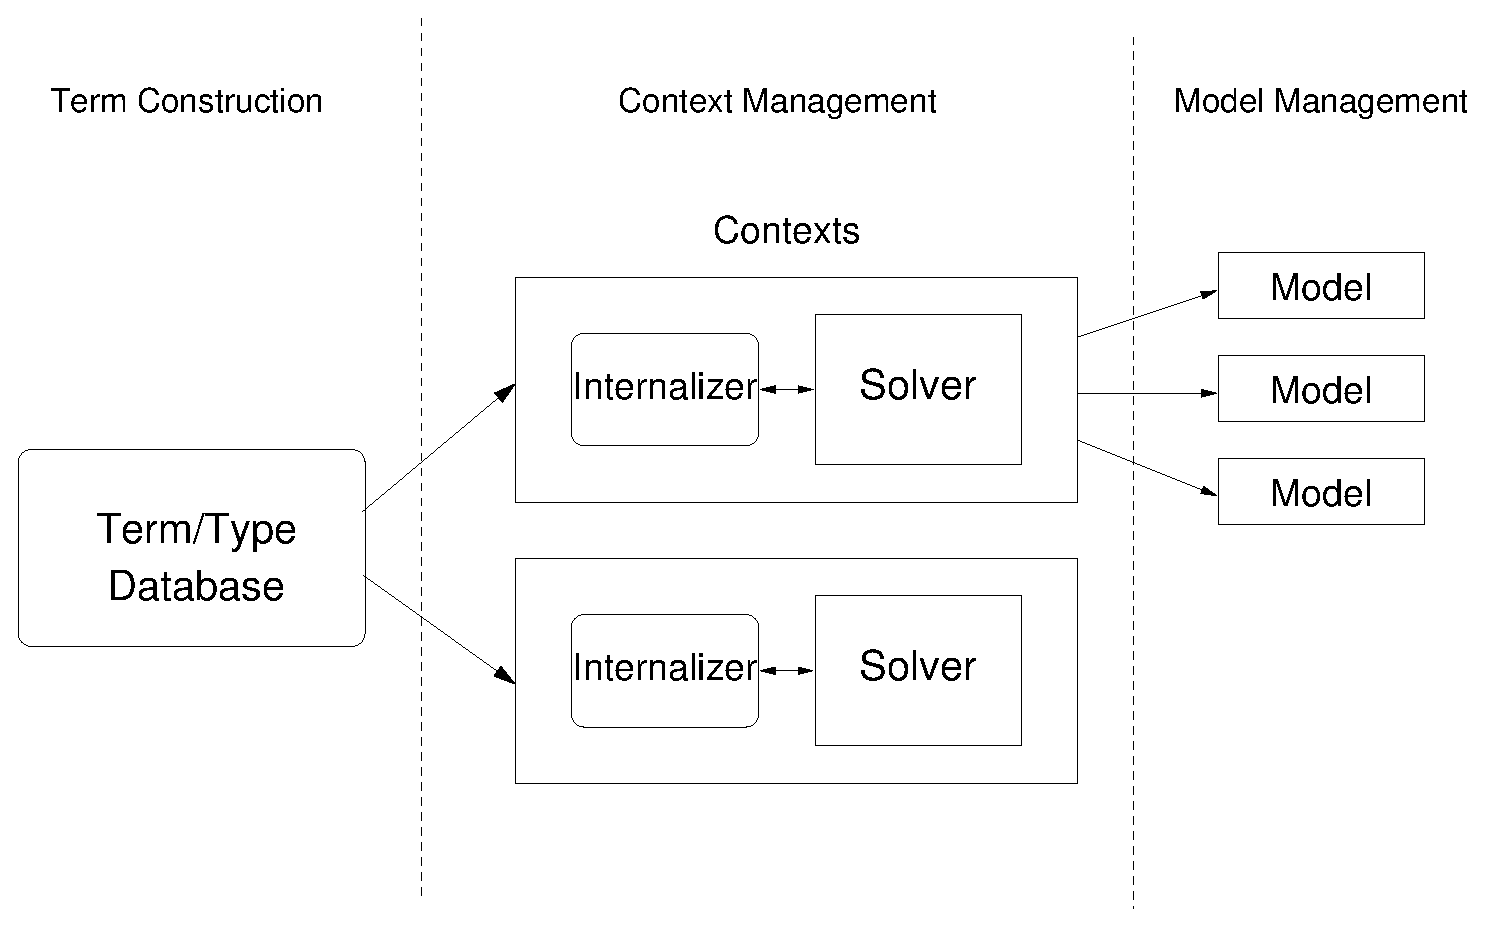
\includegraphics[width=13.8cm]{yices2-toplevel}
\caption{Top-level Yices~2 Architecture}
\label{top-level-architecture}
\end{figure}


\section{Solvers}
\label{solvers}

In Yices~2, it is possible to select a different solver (or
combination of solvers) for the problem of interest. Each context can
thus be configured for a specific class of formulas. For example, one
can use a solver specialized for linear arithmetic, or use a solver
that supports the full Yices~2
language. Figure~\ref{solver-architecture} shows the architecture of
the most general solver available in Yices~2. A major component of all
solvers is a SAT solver based on the Conflict-Driven Clause Learning
(CDCL) procedure. The SAT solver is coupled with one or more so-called
\emph{theory solvers}. Each theory solver implements a decision
procedure for a particular theory.  Currently, Yices~2 includes four
main theory solvers:
\begin{itemize}
\item The \emph{UF Solver} deals with the theory of uninterpreted
  functions with equality\footnote{UF stands for uninterpreted
    functions.}. It implements a decision procedure based on computing
  congruence closures, similar to the Simplify
  system~\cite{Detlefs-etal:JACM2005}, with other ideas borrowed
  from~\cite{Nieuwenhuis+Oliveras:UF:2007}.
\item The \emph{Arithmetic Solver} deals with linear integer and real
  arithmetic.  It implements a decision procedure based on the Simplex
  algorithm~\cite{DutertredeMoura:cav06,DutertredeMoura:report06}. 
\item The \emph{Bitvector Solver} deals with the theory of bitvectors.
\item  The \emph{Array  Solver}  implements a  decision procedure  for
  McCarthy's theory of arrays.
\end{itemize}
In addition, two arithmetic solvers can be used in place of the
Simplex-based solver for integer or real difference logic. These
solvers implement a decision procedure based on the Floyd-Warshall
algorithm. These solvers are more specialized and limited than the
Simplex-based solver. They must be used standalone; they cannot be
combined with the UF solver. 

\begin{figure}
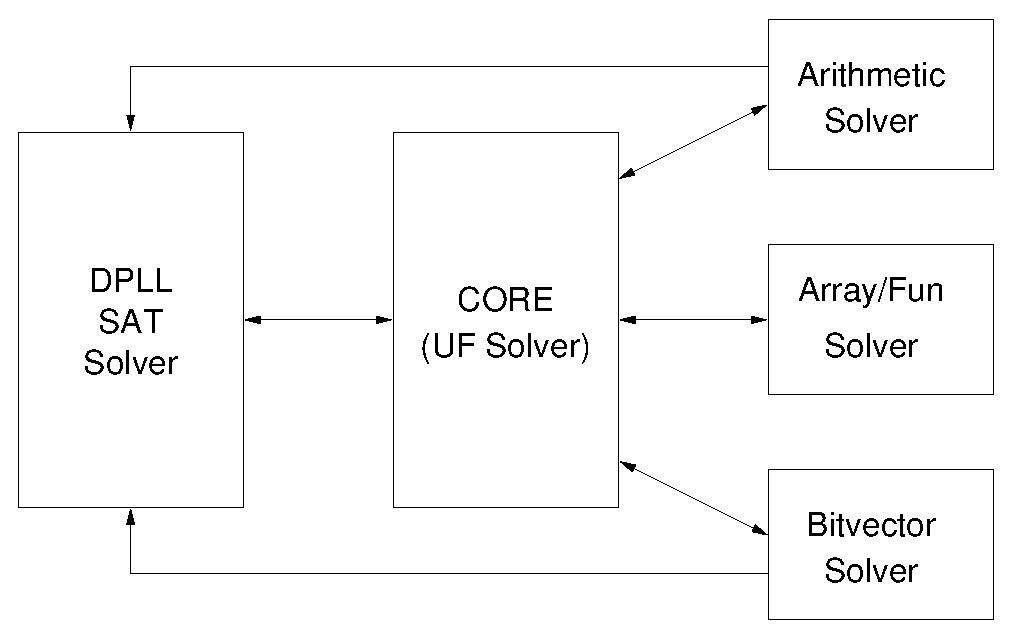
\includegraphics[width=12cm]{yices2-architecture}
\caption{Solver Components}
\label{solver-architecture}
\end{figure}


It   is    possible   to   remove   some   of    the   components   of
Figure~\ref{solver-architecture} to  build simpler and  more efficient
solvers that are specialized for  classes of formulas.  For example, a
solver  for pure  arithmetic can  be built  by directly  attaching the
arithmetic solver to  the CDCL SAT solver.  Similarly,  Yices~2 can be
specialized  for pure  bitvector problems,  or for  problems combining
uninterpreted  functions,  arrays,  and  bitvectors (by  removing  the
arithmetic solver).

Yices~2  combines   several  theory  solver   using  the  Nelson-Oppen
method~\cite{NelsonOppen79}.   The  UF solver  is  essential for  this
purpose;  it  coordinates the  different  theory  solvers and  ensures
global  consistency. The  other solvers  (for arithmetic,  arrays, and
bitvectors)  communicate only  with the  central UF  solver  and never
directly with  each other.  This property considerably  simplifies the
design and implementation of theory solvers.

\section{Context Configurations}
\label{features}

In  addition to  the set  of  solvers it  contains, a  context can  be
configured to support different  usage scenarios. The basic operations
supported by a context include:
\begin{itemize}
\item Asserting one or more formulas
\item Checking satisfiability of the set of assertions
\item Building a model if the assertions are satisfiable
\end{itemize}
In  addition, a  context can  be  configured to  support addition  and
removal of assertions  using a push/pop mechanism.  In  this case, the
context  maintains  a  stack  of assertions  organized  in  successive
levels.  The  push operation  starts a new  level and pop  removes all
assertions at the  top level.  Thus, push can be  thought as setting a
backtracking point  and pop restores  the context state to  a previous
backtracking point.

Support for  push and pop induces  some overhead and  may disable some
preprocessing and  simplification of assertions. In some  cases, it is
then desirable to  use a context without support for  push and pop, in
order to get  higher performance. Yices~2 allows users  to control the
set of  features supported by a  context by selecting  a specific {\em
  operating mode\/}.
\begin{itemize}
\item The simplest mode is {\em one-shot\/}. In this mode, one can
  assert formulas then make a one call to the check operation.
  Assertions are not allowed after the call to check. This mode is the
  most efficient as Yices may apply powerful preprocessing and
  simplification (such as symmetry breaking~\cite{Deharbe+etal:2011}).
\item The next mode is {\em multi-checks\/}. In this mode, several calls
  to the check operation are allowed. One can assert formulas, call
  check, assert more formulas and call check again. This can be done
  as long as the context is satisfiable. Once check returns
  \texttt{unsat}, then no assertions can be added. This mode avoids
  the overhead of maintaining a stack of assertions.
\item The default mode is {\em push-pop\/}. In this mode, a context
  supports the push and pop operations. Assertions are organized in a
  stack as explained previously.
\item The last mode is {\em interactive\/}. This mode provides the
  same functionalities as {\em push-pop\/}. In addition, the context
  is configured to recover gracefully when a check operation times out
  or is interrupted.
\end{itemize}



\chapter{Yices Tool}
\label{yices-shell}

The Yices~2 distribution includes  a tool for processing input written
in  the Yices~2  language.  This  tool is  called  \texttt{yices} (or
\texttt{yices.exe}  in  the Windows  and  Cygwin distributions).   The
syntax  and  the  set  of  commands supported  by  \texttt{yices}  are
explained  in  the file  \texttt{doc/YICES-LANGUAGE}  included in  the
distribution. Several example specifications  are also included in the
\texttt{examples/} directory.


\section{Example}

To      illustrate     the      tool     usage,      consider     file
\texttt{examples/bv\_test2.ys} shown in Figure~\ref{example:bv_test2}.
The  first line  defines  a  type called  \texttt{BV}.  In this  case,
\texttt{BV} is  a synonym for bitvectors  of size 32. Then  four terms
are  declared of  type \texttt{BV}.   The three  constants \texttt{a},
\texttt{b},  and \texttt{d}  are  uninterpreted,  while \texttt{c}  is
defined as  the bitvector representation  of the integer  1008832. The
next line of the file is  an assertion expressing a constraint between
\texttt{a},  \texttt{b},  \texttt{c},   and  \texttt{d}.  The  command
\texttt{(check)} checks whether the assertion is satisfiable. Since it
is, command  \texttt{(show-model)} asks for  a satisfying model  to be
displayed. The  next commands ask for  the value of four  terms in the
model.

\begin{figure}
\begin{footnotesize}
\begin{verbatim}
  (define-type BV (bitvector 32))

  (define a::BV)
  (define b::BV)
  (define c::BV (mk-bv 32 1008832))
  (define d::BV)

  (assert (= a (bv-or (bv-and (mk-bv 32 255) 
                              (bv-not (bv-or b (bv-not c)))) 
                      (bv-and c (bv-xor d (mk-bv 32 1023))))))

  (check)

  (show-model)
  (eval a)
  (eval b)
  (eval c)
  (eval d)
\end{verbatim}
\end{footnotesize}
\caption{Example Yices Script}
\label{example:bv_test2}
\end{figure}

To run \texttt{yices} on this input file, just type
\begin{small}
\begin{verbatim}
      yices examples/bv_test2.ys
\end{verbatim}
\end{small}
The tool will output something like this:
\begin{small}
\begin{verbatim}
      sat
      (= d 0b00000000000000000000000000000000)
      (= b 0b00000000000000000000000000000000)
      (= a 0b00000000000000000000000011000000)

      0b00000000000000000000000011000000
      0b00000000000000000000000000000000
      0b00000000000011110110010011000000
      0b00000000000000000000000000000000
\end{verbatim}
\end{small}
The result of the \texttt{(check)}  command is shown on the first line
(i.e., \texttt{sat}  for satisfiable). The  next three lines  show the
model as  an assignment to  the three uninterpreted  terms \texttt{a},
\texttt{b},  and \texttt{d}.  Then,  the tool  displays one  bitvector
constant for each of the \texttt{(eval ...)} command.

Since  this  example  contains  only  terms and  constructs  from  the
bitvector  theory,  we  could  specify logic  \texttt{QF\_BV}  on  the
command line as follows:
\begin{small}
\begin{verbatim}
      yices --logic=QF_BV examples/bv_test2.ys
\end{verbatim}
\end{small}
Since the file does not use \texttt{push} and \texttt{pop}, and it
contains only one call to \texttt{(check)}, one can select the mode
\texttt{one-shot}:
\begin{small}
\begin{verbatim}
      yices --logic=QF_BV --mode=one-shot examples/bv_test2.ys
\end{verbatim}
\end{small}
To get a more detailed output, give option \texttt{--verbose}:
\begin{small}
\begin{verbatim}
      yices --verbose examples/bv_test2.ys
\end{verbatim}
\end{small}

\section{Tool Invocation}

Yices is invoked on an input file by typing
\begin{verbatim}
      yices [option] <filename>
\end{verbatim}
If  no  \texttt{<filename>}  is  given,  \texttt{yices}  will  run  in
interactive  mode and  will  read the  standard  input. The  following
options are supported
\begin{description}
\item[\texttt{--logic=<name>}] Select an SMT-LIB logic.\\[1mm]
  \texttt{<name>}  must  either  be  an  SMT-LIB logic  name  such  as
  \texttt{QF\_UFLIA} or the special name \texttt{NONE}.

  Yices recognizes  the logics defined  at \url{http://www.smtlib.org}
  (as  of  December  2012).  Option  \texttt{--logic=NONE}  configures
  \texttt{yices} for propositional logic.

  By default---that is, if no logic is given---\texttt{yices} includes
  all the  theory solvers described in  Section~\ref{solvers}. In this
  default  configuration, \texttt{yices}  supports  linear arithmetic,
  bitvectors,  uninterpreted  functions, and  arrays.  If  a logic  is
  specified, \texttt{yices}  uses a specialized  solver or combination
  of  solvers that is  appropriate for  the given  logic. Some  of the
  search parameters will also be set  to values that seem to work well
  for  this logic (based  on extensive  benchmarking). All  the search
  parameters  can  also be  modified  individually  using the  command
  \texttt{(set-param ...)}.

  If  option  \texttt{--logic=NONE}   is  given,  then  \texttt{yices}
  includes no  theory solvers  at all. All  assertions must  be purely
  propositional (i.e., involve only Boolean terms).

\item[\texttt{--arith-solver=<solver>}] Select one of the possible arithmetic solvers.\\[1mm]
  \texttt{<solver>}     must    be     one     of    \texttt{simplex},
  \texttt{floyd-warshall}, or \texttt{auto}.

  If  the  logic is  \texttt{QF\_IDL}  (integer  difference logic)  or
  \texttt{QF\_RDL} (real  difference logic),  then this option  can be
  used   to  select   the  arithmetic   solver:  either   the  generic
  Simplex-based  solver   or  a   specialized  solver  based   on  the
  Floyd-Warshall algorithm.  If option \texttt{--arith-solver=auto} is
  given, then  the arithmetic solver is  determined automatically; the
  default is \texttt{auto}.

  This option has no effect  for logics other than \texttt{QF\_IDL} or
  \texttt{QF\_RDL}.

\item[\texttt{--mode=<mode>}] Select solver features.\\[1mm]
  \texttt{<mode>} can be \texttt{one-shot}, \texttt{multi-checks},
  \texttt{push-pop}, or \texttt{interactive}.

  This  option selects  the set  of functionalities  supported  by the
  solver as follows:
  \begin{itemize}
  \item   \texttt{one-shot}:   no   assertions   are   allowed   after
    \texttt{(check)},  so   only  one  call   to  \texttt{(check)}  is
    possible.
  \item \texttt{multi-checks}: several  calls to \texttt{(assert)} and
    \texttt{(check)} are allowed.
  \item \texttt{push-pop}: like \texttt{multi-checks} but with support
    for   adding   and   retracting   assertions  via   the   commands
    \texttt{(push)} and \texttt{(pop)}.
  \item  \texttt{interactive}:  supports  the  same  features  as  the
    \texttt{push-pop}  mode,  but  with   a  different  behavior  when
    \texttt{(check)} is interrupted.
  \end{itemize}
  In  the  first  two  modes, \texttt{yices}  employs  more  aggressive
  simplifications when processing assertions;  this can lead to better
  performance on some problems.

  In interactive mode,  the solver context is saved  before every call
  to  \texttt{(check)}  and  it  is restored  if  \texttt{(check)}  is
  interrupted. This introduces some  overhead, but the solver recovers
  gracefully if  \texttt{(check)} is interrupted or times  out. In the
  non-interactive modes, the solver exits after the first interruption
  or timeout.

  The default mode is \texttt{push-pop} if a file name is given on the
  command line. If  not input file is given, then  the default mode is
  \texttt{interactive} and the solver reads standard input.

  Mode \texttt{one-shot} is required if the Floyd-Warshall solvers are
  used.

\item[\texttt{--version, -V}]  Display version information then exit.

  This  displays the  Yices version  number,  the version  of the  GMP
  library  linked with  Yices, and  information about  build date  and
  platform. For example,  here is the output for  Yices~2.2.0 built on
  MacOS~X
  \begin{small}
  \begin{verbatim}
     Yices 2.2.0
     Copyright SRI International.
     Linked with GMP 5.1.3
     Copyright Free Software Foundation, Inc.
     Build date: 2013-12-21
     Platform: x86_64-apple-darwin13.0.2 (release)
  \end{verbatim}
  \end{small}
  \vspace*{-1em}
  If you ever have to report a bug, please include this version information
  in your bug report.

\item[\texttt{--help, -h}] Print a summary of options

\item[\texttt{--verbose, -v}] Run in verbose mode
\end{description}


\section{Input Language}

The   syntax  of   the   Yices  input   language   is  summarized   in
Figures~\ref{syntax:commands},~\ref{syntax:types},
and~\ref{syntax:expressions}.


\begin{figure}
\begin{small}
\begin{verbatim}
   <command>  ::= 
              ( define-type <symbol> )
            | ( define-type <symbol> <typedef> )
            | ( define <symbol> :: <type> )
            | ( define <symbol> :: <type> <expression> )
            | ( assert <expression> )
            | ( exit )
            | ( check )
            | ( push )
            | ( pop )
            | ( reset )
            | ( show-model )
            | ( eval <expression> )
            | ( echo <string> )
            | ( include <string> )
            | ( set-param <symbol> <immediate-value> )
            | ( show-param <symbol> )
            | ( show-params )
            | ( show-stats )
            | ( reset-stats )
            | ( set-timeout <number> )
            | ( show-timeout )
            | ( dump-context )
            | ( help )
            | ( help <symbol> )
            | ( help <string> )
            | EOS

   <immediate-value> ::= 
              true 
            | false
            | <number>
            | <symbol>

   <number> ::=
              <rational>
            | <float>
\end{verbatim}
\end{small}
\caption{Yices Syntax: Commands}
\label{syntax:commands}
\end{figure}  

\begin{figure}
\begin{small}
\begin{verbatim}
   <typedef> ::= 
              <type>
            | ( scalar <symbol> ... <symbol> )

   <type> ::= 
              <symbol> 
            | ( tuple <type> ... <type> )
            | ( -> <type> ... <type> <type> )
            | ( bitvector <rational> )
            | int
            | bool
            | real
\end{verbatim}
\end{small}
\caption{Yices Syntax: Types}
\label{syntax:types}
\end{figure}

\begin{figure}
\begin{small}
\begin{verbatim}
   <expr> ::= 
              true
            | false
            | <symbol>
            | <rational>
            | <float>
            | <binary bv>
            | <hexa bv>
            | ( forall ( <var_decl> ... <var_decl> ) <expr> )
            | ( exists ( <var_decl> ... <var_decl> ) <expr> )
            | ( lambda ( <var_decl> ... <var_decl> ) <expr> )
            | ( let ( <binding> ... <binding> ) <expr> )
            | ( update <expr> ( <expr> ... <expr> ) <expr> )
            | ( <function> <expr> ... <expr> )

   <function> ::=
              <function-keyword>
            | <expr>

   <var_decl> ::= <symbol> :: <type>

   <binding> ::= ( <symbol> <expr> )
\end{verbatim}
\end{small}
\caption{Yices Syntax: Expressions}
\label{syntax:expressions}
\end{figure}

\subsection{Lexical  Elements}

\subsubsection*{Comments}

Input  files  may contain  comments,  which  start  with a  semi-colon
\texttt{`;'} and extend to the end of the line.

\subsubsection*{Strings}

Strings  are similar to  strings in  C. They  are delimited  by double
quotes \texttt{"} and may contain escaped characters:
\begin{itemize}
\item     The     characters     \texttt{\textbackslash     n}     and
  \texttt{\textbackslash   t}  are  replaced   by  newline   and  tab,
  respectively.
\item The character \texttt{\textbackslash}  followed by at most three
  octal digits  (i.e., from \texttt{0}  to \texttt{7}) is  replaced by
  the character whose ASCII code is the octal number.
\item In  all other cases, \texttt{\textbackslash  <char>} is replaced
  by  \texttt{<char>} (including  if \texttt{<char>}  is a  newline or
  \texttt{\textbackslash}).
\item A  newline cannot  occur inside the  string, unless  preceded by
  \texttt{\textbackslash}.
\end{itemize}

\subsubsection*{Numerical Constants}

Numerical  constants  can  be   written  as  decimal  integers  (e.g.,
\texttt{44} or \texttt{-3}), rational (e.g., \texttt{-1/3}), or using a
floating-point  notation  (e.g.,  \texttt{0.07} or  \texttt{-1.2e+2}).
Positive  constants can start  with an  optional \texttt{+}  sign. For
example \texttt{+4} and \texttt{4} denote the same number.


\subsubsection*{Bitvector Constants}

Bitvector constants can be written in a binary format using the prefix
\texttt{0b}  or  in  hexadecimal  using the  prefix  \texttt{0x}.  For
example, the expressions  \texttt{0b01010101} and \texttt{0x55} denote
the same bitvector constant of eight bits.

\subsubsection*{Symbols}

A  symbol  is   any  character  string  that's  not   a  keyword  (see
Table~\ref{syntax:keywords}) and doesn't start  with a digit, a space,
or   one  of  the   characters  \texttt{(},   \texttt{)},  \texttt{;},
\texttt{:}, and  \texttt{"}. If the  first character is  \texttt{+} or
\texttt{-}, then it must not be  followed by a digit. Symbols end by a
space, or by any of the characters \texttt{(}, \texttt{)}, \texttt{;},
\texttt{:}, or \texttt{"}. Here are some examples:
\begin{small}
\begin{verbatim}
   a_symbol __another_one  X123  &&&  +z203  t\12
\end{verbatim}
\end{small}
All   the   predefined   keywords    and   symbols   are   listed   in
Table~\ref{syntax:keywords}.

\begin{table}
\begin{small}
\begin{center}
\begin{tt}
\begin{tabular}{|p{3.2cm}|p{3.2cm}|p{3.2cm}|}
\hline 
* & + & - \\
-> & / & /= \\
< & <= & <=> \\
 = & => & > \\
>= & \verb|^| & and \\
assert & bitvector & bool \\
bv-add & bv-and & bv-ashift-right\\
bv-ashr & bv-comp & bv-concat \\
bv-div & bv-extract & bv-ge \\
bv-gt & bv-le & bv-lshr \\
bv-lt & bv-mul & bv-nand \\
bv-neg & bv-nor & bv-not \\
bv-or & bv-pow & bv-redand \\
bv-redor & bv-rem & bv-repeat \\
bv-rotate-left & bv-rotate-right & bv-sdiv\\
bv-sge & bv-sgt & bv-shift-left0 \\
bv-shift-left1 & bv-shift-right0 & bv-shift-right1 \\
bv-shl & bv-sign-extend & bv-sle\\
 bv-slt & bv-smod & bv-srem \\
bv-sub & bv-xnor & bv-xor \\
bv-zero-extend & check & define \\
define-type & distinct & dump-context\\
echo  & eval & exists \\
exit & false & forall \\
help & if & include \\
int & ite & lambda \\
let & mk-bv & mk-tuple \\
 not & or & pop \\
push & real & reset \\
reset-stats & scalar & select \\
set-param & set-timeout & show-model \\
show-param & show-params & show-stats \\
true & tuple & tuple-update \\
update & xor &   \\
\hline
\end{tabular}
\end{tt}
\end{center}
\end{small}
\caption{Keywords and predefined symbols}
\label{syntax:keywords}
\end{table}


\subsection{Declarations}
\label{declarations}

A declaration either introduces a new type or term or gives a name to
an existing type or term. Yices uses different name spaces for types
and terms. It is then permitted to use the same name for a type and
for a term.


\subsubsection*{Type Declaration}

A type declaration is a command of the following two forms.
\begin{small}
\begin{verbatim}
   (define-type <name>)
   (define-type <name> <type>)
\end{verbatim}
\end{small}
The fist form creates a new uninterpreted type called
\texttt{<name>}. The second form gives a \texttt{<name>} to an
existing \texttt{<type>}. After this definition, every occurrence of
\texttt{<name>} refers to \texttt{<type>}. A variant of this second
form is used to define scalar types. In these two commands,
\texttt{<name>} must be a symbol that's not already used as a type
name.


\subsubsection*{Term Declaration}

A term is declared using one for the following two commands.
\begin{small}
\begin{verbatim}
   (define <name> :: <type>)
   (define <name> :: <type> <term>)
\end{verbatim}
\end{small}
The first form declares a new uninterpreted term of the given
\texttt{<type>}.  The second form assigns a \texttt{<name>} to the
given \texttt{<term>}, which must be of type \texttt{<type>}. The
\texttt{<name>} must be a symbol that's not already used as a term
name.



\subsection{Types}

Yices includes a few predefined types for arithmetic and
bitvectors. One can extend the set of atomic types by creating
uninterpreted and scalar types. In addition to the atomic types, Yices
provides constructors for tuple and function types. More details about
types and subtyping are given in Section~\ref{type-system}.

\subsubsection*{Predefined Types}

The predefined  types are \texttt{bool},  \texttt{int}, \texttt{real},
and  \texttt{(bitvector  k)} where  $k$  is  a  positive integer.  For
example a bit-vector variable \texttt{b}  of 32 bits is declared using
the command
\begin{small}
\begin{verbatim}
   (define b::(bitvector 32))
\end{verbatim}
\end{small}
The number of bits must be positive so \texttt{(bitvector 0)} is not a
valid  type.   There  is  also  a hard-coded  limit  on  the  size  of
bitvectors (namely, $2^{28}  - 1$).  Of course, this  is a theoretical
limit; the solver will most likely run out of memory if you attempt to
use bitvectors that are that large.

\subsubsection*{Uninterpreted Types}

A new uninterpreted type T can be introduced using the command
\begin{small}
\begin{verbatim}
   (define-type T)
\end{verbatim}
\end{small}
This command  will succeed provided  \texttt{T} is a fresh  type name,
that is, if there is no existing type called \texttt{T}.  As explained
in Section~\ref{type-system}, an uninterpreted type denotes a nonempty
collection  of  objects.   There   is  no  cardinality  constraint  on
\texttt{T}, except that \texttt{T} is not empty.

\subsubsection*{Scalar Type}

A scalar type is defined by enumerating its elements. For example, the
following declaration
\begin{small}
\begin{verbatim}
   (define-type P (scalar A B C))
\end{verbatim}
\end{small}
defines a  new scalar type  called \texttt{P} that contains  the three
distinct  constants  \texttt{A}, \texttt{B},  and  \texttt{C}. Such  a
declaration  is valid  provided \texttt{P}  is a  fresh type  name and
\texttt{A}, \texttt{B}, and \texttt{C} are all fresh term names.

\smallskip\noindent The enumeration must include at least one element,
but  singleton   types  are   allowed.  For  example,   the  following
declaration is valid.
\begin{small}
\begin{verbatim}
   (define-type Unit (scalar One))
\end{verbatim}
\end{small}
It introduces a  new type \texttt{Unit} of cardinality  one, and which
contains \texttt{One}  as its unique  element. Thus, any term  of type
\texttt{Unit} is known to be equal to \texttt{One}.


\subsubsection*{Tuple Types}

A tuple  type is written \texttt{(tuple <tau\_1>  ... <tau\_n>)} where
\texttt{<tau\_i>} is a type. For example, the type of pairs of integer
can be declared as follows:
\begin{small}
\begin{verbatim}
   (define-type Pairs (tuple int int))
\end{verbatim}
\end{small}
Then one can declare an uninterpreted constant \texttt{x} of this type
as follows
\begin{small}
\begin{verbatim}
   (define x::Pairs)
\end{verbatim}
\end{small}
This is equivalent to the declaration
\begin{small}
\begin{verbatim}
   (define x::(tuple int int))
\end{verbatim}
\end{small}

\smallskip\noindent   Tuple  types   with  a   single   component  are
allowed. For example, the following declaration is legal.
\begin{small}
\begin{verbatim}
   (define-type T (tuple bool))
\end{verbatim}
\end{small}

\subsubsection*{Function Types}

A function type is written \texttt{(-> <tau\_1> ...  <tau\_n>
  <sigma>)}, where $n$ is positive, and the \texttt{<tau\_i>}s and
\texttt{<sigma>} are types.  The types \texttt{<tau\_1>}, $\ldots$,
\texttt{<tau\_n>} define the domain of the function type, and
\texttt{<sigma>} is the range.  For example, a function defined over
the integers and that returns a Boolean can be declared as follows:
\begin{small}
\begin{verbatim}
   (define f::(-> int bool))
\end{verbatim}
\end{small}

\smallskip\noindent Yices does not  have a distinct type construct for
arrays. In Yices, arrays are the same as functions.


\subsection{Terms}

Yices uses a Lisp-like syntax. For example, the polynomial $x + 3y +
z$ is written
\begin{small}
\begin{verbatim}
       (+ x (* 3 y) z)
\end{verbatim}
\end{small}
In general, all associative operations can take one, two, or more
arguments. For example, one can write
\begin{small}
\begin{verbatim}
      (or A)    (or A B)    (or A B C D)
\end{verbatim}
\end{small}
since \texttt{or} is associative.


\subsubsection*{If-Then-Else}

Yices provides an if-then-else construct that applies to any type.  An
if-then-else term can be written using either one of the two following
forms
\begin{small}
\begin{verbatim}
     (ite <c> <t1> <t2>)     (if  <c> <t1> <t2>)    
\end{verbatim}
\end{small}
Both forms are equivalent and just mean ``if \texttt{<c>} then
\texttt{<t1>} else \texttt{<t2>}.''  The condition \texttt{<c>} must
be a Boolean term, and the two terms \texttt{<t1>} and \texttt{<t2>}
must have compatible types. If \texttt{<t1>} and \texttt{<t2>} have
the same type $\tau$ then \texttt{(ite <c> <t1> <t2>)} also has type
$\tau$.  Otherwise, as explained in Section~\ref{type-system}, the
type of \texttt{(if <c> <t1> <t2>)} is the minimal supertype of
\texttt{<t1>} and \texttt{<t2>}.  For example, if \texttt{<t1>} has
type \texttt{int} and \texttt{<t2>} has type \texttt{real}, then
\texttt{(ite <c> <t1> <t2>)} has type \texttt{real}.

\subsubsection*{Equalities and Disequalities}

Equalities and disequalities are written as follows
\begin{small}
\begin{verbatim}
     (=  <t1> <t2>)        (/= <t1> <t2>)
\end{verbatim}
\end{small}
where \texttt{<t1>} and \texttt{<t2>} are two terms of compatible
types. These operators are binary. Unlike SMTLIB~2, Yices does not
allow one to write \texttt{(= x y z t u)}. On the other hand, Yices
includes an $n$-ary \texttt{distinct} operator (for $n\geq 2$) that
generalizes disequality. The Boolean term
\begin{small}
\begin{verbatim}
   (distinct <t1> .... <t_n> )
\end{verbatim}
\end{small}
is true if \texttt{<t1>}, \ldots, \texttt{<t\_n>} are all different
from each other. The terms \texttt{<t1>} to \texttt{<t\_n>} must all
have compatible types. For example, \texttt{(distinct <t1> <t2>)} is
the same thing as \texttt{(/= <t1> <t2>)}. 

\subsubsection*{Boolean Operators}

\begin{table}[h]
\begin{small}
\begin{center}
\begin{tabular}{|p{2cm}|p{2cm}|}
\hline
\texttt{true} & \texttt{false} \\
\texttt{and} & \texttt{or}  \\
\texttt{not} & \texttt{xor}  \\
\texttt{<=>} & \texttt{=>}  \\
\hline
\end{tabular}
\end{center}
\end{small}
\caption{Boolean Constants and Operators}
\label{Boolean-Operators}
\end{table}


The usual Boolean constants and functions are available. They are
listed in Table~\ref{Boolean-Operators}.  The associative/commutative
operators \texttt{or}, \texttt{and}, and \texttt{xor} can take any
number of arguments. The equivalence (\texttt{<=>}) and implication
(\texttt{=>}) operators take exactly two arguments.

One can also use the equality and disequality operators
with Boolean terms. If \texttt{<t1>} and \texttt{<t2>} are Boolean
then \texttt{(= <t1> <t2>)} is the same as \texttt{(<=> <t1> <t2>)},
and \texttt{(/= <t1> <t2>)} is the same as \texttt{(xor <t1> <t2>)}.

\subsubsection*{Arithmetic}

Arithmetic constants can be written in decimal, as rationals, or using
floating point notation. Internally, Yices uses exact rational
arithmetic and it represents all arithmetic constants as rationals.

\begin{table}[h]
\begin{small}
\begin{center}
\begin{tabular}{|p{4cm}|l|c|}
\hline
Syntax & \multicolumn{2}{|c|}{Meaning} \\
\hline
\texttt{(+ a1 ... a\_n)} & sum & $a_1 + \ldots + a_n$ \\
\texttt{(* a1 ... a\_n)} & product & $a_1 \times \ldots \times a_n$ \\
\texttt{(- a)} & opposite & $-a$\\
\texttt{(- a1 a2 ... a\_n)} & difference &  $a_1 - a_2 - \ldots - a_n$ \\
\texttt{(\char`\^\  a k)} & exponentiation & $a^k$ \\
\texttt{(/ a c)} & division & $a/c$ \\
\hline 
\texttt{(<= a1 a2)} & inequality & $a_1 \leq a_2$\\
\texttt{(>= a1 a2)} & inequality & $a_1 \geq a_2$\\
\texttt{(< a1 a2)} & strict inequality & $a_1 < a_2$ \\
\texttt{(> a1 a2)} & strict inequality & $a_1 > a_2$ \\
\hline
\end{tabular}
\end{center}
\end{small}
\caption{Arithmetic Operations}
\label{Arithmetic-Operations}
\end{table}

The usual arithmetic operations and comparison operators are
summarized in Table~\ref{Arithmetic-Operations}. One can freely mix
terms of real and integer types in all operations. The exponent $k$ in
\texttt{(\char`\^\ a k)} must be a non-negative integer constant. The
divisor \texttt{c} in \texttt{(/ a c)} must be a non-zero constant.

The Yices language includes more than linear arithmetic, but this is
for future extensions. Currently, Yices does not include solvers for
non-linear arithmetic (cf. Sect.~\ref{solvers}).

\subsubsection*{Bitvectors Constants}

A bitvector constant can be written in binary or hexadecimal notation, as follows
\begin{small}
\begin{verbatim}
   0b0   0b1   0xFFFF    0xaaaa    0xC0C0D0D0
\end{verbatim}
\end{small}
In the binary notation, the number of bits in the constant is equal to
be number of binary digits. For example, the three terms
\begin{small}
\begin{verbatim}
   0b1   0b0001   0b00001
\end{verbatim}
\end{small}
denote distinct bitvector constants, of one, four, and five bits, respectively.
In the hexadecimal notation, the number of bits is equal to four times the number
of hexadecimal digit.

One can also construct a bitvector constant using the expression:
\begin{small}
\begin{verbatim}
   (mk-bv <size> <value>)
\end{verbatim}
\end{small}
In this expression, both \texttt{<size>} and \texttt{<value>} must be
integer constants; \texttt{<size>} is the number of bits in the
bitvector constant and \texttt{<value>} is the decimal value of the
constant interpreted as a non-negative integer. The \texttt{<size>}
must then be positive, and the \texttt{<value>} must be
non-negative. If \texttt{<value>} is more than $2^{\mathtt{size}}$,
only the residue of \texttt{<value>} modulo $2^{\mathtt{size}}$ is
taken into account. For example, the expressions
\begin{small}
\begin{verbatim}
   (mk-bv 3 6)    (mk-bv 3 22)
\end{verbatim}
\end{small}
construct the same bitvector constant (whose binary representation is
\texttt{0b110}).

\subsubsection*{Bitvector Arithmetic}

\begin{table}
\begin{small}
\begin{center}
\begin{tabular}{|p{5cm}|l|}
\hline Syntax & Meaning \\ \hline \texttt{(bv-add u1 ... u\_n)} & sum
\\ \texttt{(bv-mul u1 ... u\_n)} & product \\ \texttt{(bv-sub u1
  ... u\_n)} & subtraction \\ \texttt{(bv-neg u)} & 2s-complement
\\ \texttt{(bv-pow u k)} & exponentiation \\ \hline \texttt{(bv-not
  u)} & bitwise complement \\ \texttt{(bv-and u1 ... u\_n)} & bitwise
and \\ \texttt{(bv-or u1 ... u\_n)} & bitwise or \\ \texttt{(bv-xor u1
  ... u\_n)} & bitwise xor \\ \texttt{(bv-nand u1 ... u\_n)} & bitwise
nand \\ \texttt{(bv-nor u1 ... u\_n)} & bitwise nor
\\ \texttt{(bv-xnor u1 ... u\_n)} & bitwise xnor \\ \hline
\end{tabular}
\end{center}
\end{small}
\caption{Bitvector Operations (Arithmetic and Bitwise Logic)}
\label{bitvectors1}
\end{table}

Table~\ref{bitvectors1} lists all the arithmetic and bitwise
operators. All operators in this table take arguments that have the
same size and return a result of that size.  As usual, the associative
operators can take one, two, or more arguments. The \texttt{bv-sub}
operator takes at least two arguments. In \texttt{(bv-pow u k)},
the power $k$ must be a non-negative integer constant. 

The expression \texttt{(bv-xnor u1 ... u\_n)} is the same as
\texttt{(bv-not (bv-xor u1 ... u\_n))}.

\subsubsection*{Bitvector Shift and Rotate}

\begin{table}
\begin{small}
\begin{center}
\begin{tabular}{|p{5cm}|l|}
\hline
Syntax & Meaning \\
\hline
\texttt{(bv-shift-left0 u k)} & left shift, padding with 0\\
\texttt{(bv-shift-left1 u k)} & left shift, padding with 1\\
\texttt{(bv-shift-right0 u k)} & right shift, padding with 0\\
\texttt{(bv-shift-right1 u k)} & right shift, padding with 1\\
\texttt{(bv-ashift-right x k)} &  arithmetic shift by $k$ bits\\
\texttt{(bv-rotate-left x k)} & rotate by $k$ bits to the left\\
\texttt{(bv-rotate-right x k)} & rotate by $k$ bits to the right\\
\hline
\texttt{(bv-shl u v)} & left shift (padding with 0)\\
\texttt{(bv-lshr u v)} & logical right shift (padding with 0) \\
\texttt{(bv-ashr u v)} & arithmetic shift (padding with the sign bit)\\
\hline
\end{tabular}
\end{center}
\end{small}
\caption{Bitvector Operations (Shift and Rotate)}
\label{bitvectors2}
\end{table}

Table~\ref{bitvectors2} lists the shift and rotate operations. The
operations in the first seven rows shift a bitvector \texttt{u} by a
fixed number of bits $k$. If \texttt{u} is a bitvector of $n$ bits,
then $k$ must be an integer constant such that $0 \leq k \leq n$. The
\texttt{bv-shl}, \texttt{bv-lshr}, and \texttt{bv-ashr} operators
(last three rows of Table~\ref{bitvectors2}) take two bitvector
arguments \texttt{u} and \texttt{v}, which must be bitvectors of the
same size $n$. The shift operation is applied to \texttt{u}; the value
of \texttt{v}, interpreted as an unsigned integer in the range $[0,
  2^n-1]$, defines the shift amount. The semantics follows the SMT-LIB
standards: if \texttt{v}'s value is more than $n$ then the padding bit
is copied $n$ times.

\subsubsection*{Bitvector Structural Operations}

\begin{table}
\begin{small}
\begin{center}
\begin{tabular}{|p{5cm}|l|}
\hline
Syntax & Meaning \\
\hline
\texttt{(bv-extract i j u)} & subvector extraction \\
\texttt{(bv-concat u1 ... u\_n)} & concatenation \\
\texttt{(bv-repeat u k)} & repeated concatenation \\
\texttt{(bv-sign-extend u k)} & sign extension \\
\texttt{(bv-zero-extend u k)} & zero extension \\
\hline
\texttt{(bv-redor u)} & or-reduction \\
\texttt{(bv-redand u)} & and-reduction \\
\texttt{(bv-redcomp u v)} & equality reduction \\
\hline
\end{tabular}
\end{center}
\end{small}
\caption{Bitvector Operations (Structural Operators)}
\label{bitvectors3}
\end{table}

The operators in Table~\ref{bitvectors3} perform extraction,
concatenation, and other structural operations. The expression
\texttt{(bv-extract i j u)} is the segment of bitvector \texttt{u}
formed by taking bits $j, j+1, \ldots, i$. If \texttt{u} is a
bitvector of $n$ bits then the constants $i$ and $j$ must satisfy $0
\leq j \leq i \leq n-1$, and the result is a bitvector of $(i - j +
1)$ bits. For example, we have
\begin{small}
\begin{verbatim}
   (bv-extract 7 2 0b110110100) = 0b101101.
\end{verbatim}
\end{small}

In \texttt{(bv-repeat u k)}, bitvector \texttt{u} is concatenated with
itself $k$ times. The integer constant $k$ must be positive. In the
sign and zero extension operators, vector \texttt{u} is extended by
adding $k$ bits (either zero or \texttt{u}'s sign bit copied $k$
times).  In these two operations, $k$ must be non-negative.

The \texttt{bv-redor}, \texttt{bv-redand}, and \texttt{bv-redcomp}
operators produce a one-bit vector.  The term \texttt{(bv-redor u)} is
the or of \texttt{u}'s bits; it is equal to \texttt{0b0} if all bits
of \texttt{u} are zero, and to \texttt{0b1} otherwise. Similarly,
\texttt{(bv-redand u)} is the and of \texttt{u}'s bit; it is equal to
\texttt{0b1} if all bits of \texttt{u} are one and to \texttt{0b0}
otherwise. In \texttt{(bv-redcomp u v)}, the arguments \texttt{u} and
\texttt{v} must be two bitvectors of the same size. The operator
performs a one-to-one comparison of the bits of \texttt{u} and
\texttt{v} and returns either \texttt{0b1}, if \texttt{u} and
\texttt{v} are equal, or \texttt{0b0}, if \texttt{u} and \texttt{v}
are distinct.

\subsubsection*{Bitvector Division}

\begin{table}
\begin{small}
\begin{center}
\begin{tabular}{|p{3.3cm}|l|}
\hline
Syntax & Meaning \\
\hline
\texttt{(bv-div u v)} & quotient in unsigned division \\
\texttt{(bv-rem u v)} & remainder in unsigned division \\
\hline
\texttt{(bv-sdiv u v)} & quotient in signed division \\
\texttt{(bv-srem u v)} & remainder in signed division \\
\hline
\texttt{(bv-smod u v)} & remainder in signed division (rounding to $-\infty$)\\
\hline
\end{tabular}
\end{center}
\end{small}
\caption{Bitvector Operations (Divisions)}
\label{bitvectors4}
\end{table}

Table~\ref{bitvectors4} lists the division and remainder operators. In
this table, \texttt{u} and \texttt{v} must be two bitvectors of the
same size $n$. 

In the unsigned division and quotient operations, \texttt{u} and
\texttt{v} are interpreted as integers in the interval $[0,2^n-1]$.
As explained in section~\ref{bitvector-general}, \texttt{(bv-div u v)}
is the largest integer that can be represented using $n$ bits and is
smaller than or equal to $\frac{u}{v}$. The unsigned remainder
\texttt{(bv-rem u v)} satisfies the identity
\begin{small}
\begin{verbatim}
  u = (bv-add (bv-mul (bv-div u v) v) (bv-rem u v)).
\end{verbatim}
\end{small}
In the signed division and quotient, \texttt{u} and \texttt{v} are
interpreted as integers in the interval $[-2^{n-1},2^{n-1}-1]$ (in
2s-complement representation), and the division is done with rounding
to zero. 
\begin{itemize}
\item If $\frac{u}{v}$ is non-negative, then \texttt{(bv-sdiv u v)}
is the largest integer $q$ in $[0,2^{n-1}-1]$ such that $0 \leq q \leq
\frac{u}{v}$. 
\item If $\frac{u}{v}$ is negative then \texttt{(bv-sdiv u v)}
is the smallest integer $q$ in $[-2^{n-1}, 0]$ such that $\frac{u}{v}
\leq q \leq 0$.
\end{itemize}
The signed remainder operation satisfies the identity
\begin{small}
\begin{verbatim}
  u = (bv-add (bv-mul (bv-sdiv u v) v) (bv-srem u v)).
\end{verbatim}
\end{small}
The last operator in Table~\ref{bitvectors4} is the remainder in the
signed division of \texttt{u} by \texttt{v} with rounding to
$-\infty$.  In this operation, \texttt{u} and \texttt{v} are
interpreted as signed integers in the interval $[-2^{n-1},2^{n-1}-1]$;
the quotient is $\lfloor \frac{u}{v} \rfloor$ (i.e., the largest
integer $q$ such that $q \leq \frac{u}{v}$); and the remainder is $u -
q v$. The special case $v=0$ is explained in
Section~\ref{bitvector-general}.

\subsubsection*{Bitvector Inequalities}

\begin{table}
\begin{small}
\begin{center}
\begin{tabular}{|p{3cm}|l|}
\hline
Syntax & Meaning \\
\hline
\texttt{(bv-ge u v)} & $u \geq v$ unsigned\\
\texttt{(bv-gt u v)} & $u > v$ unsigned \\
\texttt{(bv-le u v)} & $u \leq v$ unsigned \\
\texttt{(bv-lt u v)} & $u < v$ unsigned \\
\hline
\texttt{(bv-sge u v)} & $u \geq v$ signed\\
\texttt{(bv-sgt u v)} & $u > v$ signed \\
\texttt{(bv-sle u v)} & $u \leq v$ signed \\
\texttt{(bv-slt u v)} & $u < v$ signed \\
\hline
\end{tabular}
\end{center}
\end{small}
\caption{Bitvector Operations (Comparison)}
\label{bitvectors5}
\end{table}

Table~\ref{bitvectors5} lists the inequality comparison operators for
bitvectors. In the table, \texttt{u} and \texttt{v} must be two
bitvector terms of the same size. Depending on the operation, both are
interpreted as unsigned integers or as signed integers (using
2s-complement representation).  All operators return a Boolean. As
usual, one can also apply the equality and disequality operators to
two bitvectors of the same size. 


\subsubsection*{Tuples}

A tuple term can be constructed using \texttt{(mk-tuple t1 ... t\_n)}
where $n\geq1$ and \texttt{t1}, \ldots, \texttt{t\_n} are arbitrary
terms. For example, a pair of integers can be constructed using
\begin{small}
\begin{verbatim}
   (mk-tuple -1 1)
\end{verbatim}
\end{small}

\smallskip\noindent The projection operation extracts the $i$-th
component of a tuple. It is denoted by \texttt{(select t i)} where
\texttt{t} is a term of tuple type and $i$ is an integer constant.  If
the tuple has $n$ components, then $i$ must be between $1$ and
$n$. The components are indexed from 1 to $n$ starting from the
left. For example, we have
\begin{small}
\begin{verbatim}
   (select (mk-tuple -1 1) 1) = -1
   (select (mk-tuple -1 1) 2) = 1
\end{verbatim}
\end{small}

\smallskip\noindent Yices includes a tuple-update operator. The expression
\texttt{(tuple-update t i v)} is equal to tuple \texttt{t} with its $i$-th
component replaced by \texttt{v}. The type of \texttt{v} must be a subtype of 
the $i$-th component of \texttt{t}.

\subsubsection*{Function Updates}

Array or function update is written \texttt{(update a (i1 ... i\_n)
  v)}. In this expression, \texttt{a} must be a term with a function
type and $n$ is the arity of \texttt{a}. The expression constructs a
function \texttt{b} that is equal to \texttt{a}, except that it maps
\texttt{i1},\ldots,\texttt{i\_n} to \texttt{v}.  The semantics and
typechecking rules of this operator are explained in
Section~\ref{terms-and-formulas}.


\subsection{Commands}

The Yices commands allows one to  declare types and terms, build a set
of  assertions, check  their  satisfiability, and  query models.  Other
commands set parameters that control preprocessing and heuristics used
by the different solvers.

\subsubsection*{Declarations}

As presented in Section~\ref{declarations}, Yices provides two
commands for declaring types and terms.  A type declaration has the
one of the following form
\begin{small}
\begin{verbatim}
   (define-type <name>)
   (define-type <name> <type>)
\end{verbatim}
\end{small}
A term declaration is similar:
\begin{small}
\begin{verbatim}
   (define <name> :: <type>)
   (define <name> :: <type> <term>)
\end{verbatim}
\end{small}
To define a function, one can use the \texttt{lambda} notation.  Here
is an example:
\begin{small}
\begin{verbatim}
   (define max::(-> real real real)
      (lambda (x::real y::real) (if (< x y) y x)))
\end{verbatim}
\end{small}
This defines the function \texttt{max} that computes the maximum of
two real numbers. Note that such a function definition acts like a
macro. A term of the form \texttt{(max a b)} is eagerly replaced by
the ``function body'', that is, by the term \texttt{(if (< a b) b a)}.
The ability to define function is useful to abbreviate specifications,
but it must be used with care. Since the substitution is performed
eagerly, the expanded terms may grow quickly, especially if they
contain nested function applications.


All declarations have global scope and are permanent. They are not
affected by commands such as push, pop, or reset. Also, as discussed
previously, Yices uses separate name spaces for terms and for types.



\subsubsection*{Assertions}

The following command adds an assertion to the current context.
\begin{small}
\begin{verbatim}
   (assert <formula>)
\end{verbatim}
\end{small}
In this command, the \texttt{<formula>} must be a Boolean term. 

\medskip

In the mode \texttt{one-shot}, assertions are stored internally and
are not processed immediately. Processing of assertions is delayed,
and all assertions are processed and simplified on the first call to
\texttt{(check)}.

In all other modes, the assertions are processed and simplified
immediately and are added to the context. As a result, \texttt{yices}
may detect and report that the current set of assertions is
inconsistent after an \texttt{assert} command. This happens when the
context is seen to be unsatisfiable by simplification only. The most
trivial example is:
\begin{small}
\begin{verbatim}
   (assert false)   
\end{verbatim}
\end{small}
Once the context is unsatisfiable, new assertions are treated as an
error.


\subsubsection*{Check}

The command
\begin{small}
\begin{verbatim}
   (check)
\end{verbatim}
\end{small}
checks whether the current set of assertions is satisfiable. 

\medskip

If the context's current status is already known, then the command
returns immediately and prints the status as either \texttt{sat} or
\texttt{unsat}. This happens, for example, in the following situation:
\begin{small}
\begin{verbatim}
   (assert ...)
   (check)
   (check)
\end{verbatim}
\end{small}
The context status is known after the first \texttt{(check)} command
(provided this command does not timeout or otherwise fails). Then the
second \texttt{(check)} does nothing and just prints the current
status.

If the context's status is unknown, then \texttt{(check)} invokes the
SMT solver to establish whether the assertions are satisfiable. As
discussed previously, the actual solver or solver combination is
dependent on command-line options given to the \texttt{yices} tool. In
particular, the \texttt{--logic} option allows one to select a solver
architecture that is specialized for a particular logic. For best
performance, it is usually better to specify the logic if it is known
in advance.

Several  heuristic parameters  can also  control some  aspects  of the
search algorithm  employed by the solver. Yices  use default settings
based  on the  specified  logic (or  global  defaults if  no logic  is
given). All these  parameters can be examined and  modified, using the
command  \texttt{show-params} and  \texttt{set-param}  described in  a
subsequent section.

One can also provide a timeout before calling \texttt{(check)}. If the
timeout is reached or the search is interrupted (by CTRL-C), then the
result will be displayed as \texttt{interrupted}. 


\subsubsection*{Push, Pop, Reset}

Command \texttt{(push)}, \texttt{(pop)}, and \texttt{(reset)} allows
one to manipulate the set of assertions. 

\medskip

The command \texttt{(reset)} clears all assertions. The current
context is then returned to its initial state, where the set of
assertions is empty. This command can be used in all modes.

The push and pop commands are supported by \texttt{yices} if it is run
in mode \texttt{push-pop} or \texttt{interactive}. In these modes, the
context maintains a stack of assertions organized in successive
levels. The \texttt{(push)} command starts a new assertion level in
this stack, and \texttt{(pop)} removes all assertions at the current
level. The command \texttt{(assert f)} adds an assertion \texttt{f} to
the current level. This assertion will be part of the context until
this current level is exited by either a call to \texttt{(pop)} or a
call to \texttt{(reset)}. Thus, a call to \texttt{(pop)} retracts all
assertions entered since the matching \texttt{(push)}.  The initial
assertion level includes all formulas that are asserted before the
first \texttt{(push)} command. Such assertions cannot be retracted by
\texttt{(pop)}. They remain in the context until \texttt{(reset)} is
called.

The commands \texttt{(reset)} and \texttt{(pop)} modify the set of
assertions in the context, but they do not affect term and type
declarations. For example, the following sequence of commands is
valid.
\begin{small}
\begin{verbatim}
   (push)
   (define A::bool)
   (assert A)
   (check)
   (pop)
   (assert (not A))
   (check)   
\end{verbatim}
\end{small}
The term \texttt{A} is declared after the \texttt{(push)} command. The
\texttt{(pop}) command removes the first assertion but its does not
remove the declaration. Thus, \texttt{A} remains declared as a Boolean
term after the \texttt{(pop)} command. The second assertion is then
valid. Both calls to \texttt{(check)} return \texttt{sat}.


\subsubsection*{Model}

If a call to \texttt{(check)} returns \texttt{sat}, then the set of
assertions in the context is satisfiable. One can request
\texttt{yices} to construct and display a model for the
assertions. One can also evaluate the value of arbitrary terms in this
model.

\medskip

The command
\begin{small}
\begin{verbatim}
   (show-model)
\end{verbatim}
\end{small}
displays the current model (and constructs it if necessary). An error
is reported if the context's status is unknown or if the context is
not satisfiable. Otherwise, the model is displayed in the format
illustrated in Figure~\ref{model-format}. The model is displayed as a
list of assignments, possibly followed by a list of function
definitions. An assignment has the form
\begin{small}
\begin{verbatim}
   (= <name> <value>)
\end{verbatim}
\end{small}
where \texttt{<name>} is an uninterpreted constant and
\texttt{<value>} is a constant, that is, the value mapped to
\texttt{<name>} in the model. This format is used for all terms of
atomic types (Boolean, integer and real, bitvector, scalar, and
uninterpreted types). It is also used to display the value of terms
that have tuple type. The value of an uninterpreted functions $f$ is
displayed as shown on the right column of Figure~\ref{model-format}.
For each uninterpreted function, \texttt{yices} displays the type of
the function, a finite list of assignments, and the function's default
value. For example, in Figure~\ref{model-format}, one can see that
\texttt{yices} has constructed a model where \texttt{(b 0)} and
\texttt{(b 1)} are \texttt{true}, and the default value for \texttt{b}
is \texttt{false}.  This means that \texttt{(b x)} is \texttt{false}
for any \texttt{x} different from \texttt{0} and \texttt{1}.

\begin{figure}
\begin{footnotesize}
\begin{center}
\begin{tabular}{c|c}
\multicolumn{1}{c}{Input} & \multicolumn{1}{c}{Model} \\[0.4em]

\begin{minipage}[t]{6cm}
\begin{verbatim}
(define a::(-> int bool))
(define b::(-> int bool))
(define c::(-> int bool))
(define x::int)
(define y::int)
(assert (and (a x) (b y)))
(assert (/= x y))
(assert (distinct a b c))
(check)
(show-model)
\end{verbatim}
\end{minipage}~~
&
~~~\begin{minipage}[t]{6cm}
\begin{verbatim}
(= y 0)
(= x -579)
(function c
 (type (-> int bool))
 (default true))
(function a
 (type (-> int bool))
 (= (a 1) false)
 (default true))
(function b
 (type (-> int bool))
  (= (b 0) true)
  (= (b 1) true)
  (default false))
\end{verbatim}
\end{minipage}
\end{tabular}
\end{center}
\end{footnotesize}
\caption{Model Display Format}
\label{model-format}
\end{figure}

\pagebreak

Command
\begin{small}
\begin{verbatim}
   (eval <term>)
\end{verbatim}
\end{small}
computes the value assigned to \texttt{<term>} in the current model,
and displays this value. For example, assuming the model shown in 
Figure~\ref{model-format}, one can type
\begin{small}
\begin{verbatim}
   (eval (a y))
\end{verbatim}
\end{small}
and the result will be \texttt{true}. It is also possible to ask for
the value of a function term, as in
\begin{small}
\begin{verbatim}
   (eval (update a (y) false))
\end{verbatim}
\end{small}
The result is displayed as a function specification such as:
\begin{small}
\begin{verbatim}
   (function fun!17
     (type (-> int bool))
     (= (fun!17 1) false)
     (= (fun!17 0) false)
     (default true))
\end{verbatim}
\end{small}
Yices creates an internal name of the form \texttt{fun!<number>} to
display the function value.

\subsubsection*{Parameters}

A number of parameters control the preprocessing and simplifications
applied by Yices, and the heuristics used by the CDCL SAT solver and the
theory solvers. Several commands allow one to examine and modify these
parameters.

To see the list of all available parameters, and their current values, type
\begin{small}
\begin{verbatim}
   (show-params)
\end{verbatim}
\end{small}
If you want to see the value of a specific parameter, type
\begin{small}
\begin{verbatim}
   (show-param <name>)
\end{verbatim}
\end{small}
where \texttt{<name>} is the parameter name. To set a parameter value, use
\begin{small}
\begin{verbatim}
    (set-param <name> <value>)
\end{verbatim}
\end{small}
For example, the CDCL solver can use different branching
heuristics. This is controlled by the \texttt{branching} parameter. To
see its current value, type the command
\begin{small}
\begin{verbatim}
   (show-param branching)
\end{verbatim}
\end{small}
To select a branching heuristic, use a command like
\begin{small}
\begin{verbatim}
   (set-param branching negative)
\end{verbatim}
\end{small}
 
There are many search and preprocessing parameters. The full list is
described in the file \texttt{doc/YICES-LANGUAGE} included in the
distribution. You can also get on-line help on the parameter using 
\begin{small}
\begin{verbatim}
   (help params)
\end{verbatim}
\end{small}
One can also get on-line help on a specific parameter. For example,
the command
\begin{small}
\begin{verbatim}
   (help branching)
\end{verbatim}
\end{small}
will print a short description of the parameter \texttt{branching} and
list its possible values.

\subsubsection*{Timeout}

By default, \texttt{yices} does not use a timeout. So a call to
\texttt{(check)} may take a very long time to terminate. To limit the
runtime of \texttt{(check)}, one can give a timeout is seconds. For
example, to limit the runtime to 2 minutes:
\begin{small}
\begin{verbatim}
   (set-timeout 120)
\end{verbatim}
\end{small}
This timeout will apply to the next call to \texttt{(check)}, but not
to the one after that. After every call to \texttt{(check)}, the
timeout is rest to 0 (which means no timeout). One can also clear the 
timeout explicitly by setting it to 0:
\begin{small}
\begin{verbatim}
   (set-timeout 0)
\end{verbatim}
\end{small}
To see the current value of the timeout, one can use the command
\begin{small}
\begin{verbatim}
   (show-timeout)
\end{verbatim}
\end{small}

\subsubsection*{Echo}

The \texttt{echo} command can be use to print a string on the standard
output. It can be useful in Yices scripts to help display
results. An example in Figure~\ref{example-echo} illustrates its use.

\begin{figure}
\begin{center}
\begin{footnotesize}
\begin{verbatim}
    (define a::bool)
    (define b::bool)
    (define c::bool)
    (define d::bool)
    (define e::bool)

    (assert (= a (or b c)))
    (assert (= d (and b c)))
    (assert (= a d))
    (echo "First check: should be sat\n")
    (check)
    (show-model)

    (assert (= e (xor b c)))
    (assert (= e d))
    (echo "\nSecond check: should be sat\n")
    (check)
    (show-model)

    (assert d)
    (echo "\nThird check: should be unsat\n")
    (check)
\end{verbatim}
\end{footnotesize}
\end{center}
\caption{Example Use of the \texttt{echo} Command}
\label{example-echo}
\end{figure}

\subsubsection*{Include}

It is possible to include a Yices script using the following command:
\begin{small}
\begin{verbatim}
   (include <filename>)
\end{verbatim}
\end{small}
where \texttt{<filename>} is the name of an input file given as a
string. For example, to include the file \texttt{example.ys}, type
\begin{small}
\begin{verbatim}
   (include "example.ys")
\end{verbatim}
\end{small}
This command will read and execute all commands contained in the given
file.

\subsubsection*{Help}

The \texttt{yices} tool has on-line help, which can be obtained using one
of the following commands:
\begin{small}
\begin{verbatim}
   (help)
   (help <topic>)
\end{verbatim}
\end{small}
Without argument, \texttt{(help)} prints a summary of the main Yices
  commands. With an argument, \texttt{(help <topic>)} gives help on
  the specified \texttt{<topic>}. The argument can be a command name,
  one of the built-in type or term constructor, or the name of an
  parameter.  The argument can be given as a string or as a
  symbol. For example, to get some information on the search parameter \texttt{var-elim},
one can type either
\begin{small}
\begin{verbatim}
   (help "var-elim")
\end{verbatim}
\end{small}
or just 
\begin{small}
\begin{verbatim}
   (help var-elim).
\end{verbatim}
\end{small}
On-line help is available for other topics such as the syntax. To get a
list of all topics, one can type
\begin{small}
\begin{verbatim}
   (help index)
\end{verbatim}
\end{small}


\subsubsection*{Statistics}

The solver keeps track of various statistics concerning the search
algorithms (e.g., the number of decisions and conflicts in the CDCL
solver). The following command prints all the internal statistics
\begin{small}
\begin{verbatim}
   (show-stats)
\end{verbatim}
\end{small}
As part of these statistics, \texttt{yices} keeps track of the
cumulative CPU time spent in calls to the \texttt{check} command.  To
get time measurement for a specific call to \texttt{(check)} (rather
than the total amount of time spent on all calls to \texttt{(check)}
so far), one can reset the global time counter to zero using command
\texttt{(reset-stats)}. To get the runtime and other statistics about
a specific \texttt{(check)}, type the following commands:
\begin{small}
\begin{verbatim}
   (reset-stats)
   (check)
   (show-stats)
\end{verbatim}
\end{small}

\subsubsection*{Exit}

At any time, one can exit the solver using the command
\begin{small}
\begin{verbatim}
   (exit)
\end{verbatim}
\end{small}
If this command is part of a Yices script file, then \texttt{yices}
exits immediately after this command, without parsing or processing the
rest of the file.


% 4) Built-in constants and functions
%    --------------------------------

% 4.1) ite is the if-then-else construct. 
%      if is a synonym for ite

%      distinct takes at least 2 arguments.

%      =, /= are strictly binary (unlike in SMT-LIB 1, where = can take more than two arguments).


% 4.2) true, false, or, and, not, xor, <=>, => are the usual boolean constants and 
%      functions.
     
%      or, and, xor can take any number of arguments (provided there's at least one).

%      <=> and => are binary operators.


% 4.3) tuple constructor: (mk-tuple <term_1> ... <term_n>) with n>=1

%      projection: (select <tuple> i) is the i-th component of term
%           <tuple> must have type (tuple tau_1 ... tau_n) 
%       and i must be between 1 and n
 
%      tuple update: (tuple-update <tuple> i <term>) is <tuple> with 
%      the i-th component replaced by <term>


% 4.4) function update: (update <function> (<arg_1> ... <arg_n>) <new_value>)


% 4.5) bitvector functions:

%      a) bitvector constant from an integer

%         (mk-bv <size> <value>)

%         Note: value must be a non-negative integer and 
%         size must be a positive integer.


%      b) bitvector arithmetic

%         bv-add, bv-sub, bv-mul take exactly two arguments, and both 
% 	must have the same size     

%         (bv-neg x) = opposite of x in 2's complement arithmetic

%         (bv-pow x k) = exponentiation (k must be a non-negative integer constant)


%      c) bitwise logical operators

%         (bv-not x) = bitwise negation of x

%         bv-and, bv-or, bv-xor, bv-nand, bv-nor, bv-xnor: bitwise operators,
%         all take two arguments of the same size

%         note: (bv-xnor x y) is the same as (bv-not (bv-xor x y)).


%      d) shift/rotate by a fixed constant

%         (bv-shift-left0 x k):  shift x by k bits to the left, padding with 0
%         (bv-shift-left1 x k):  shift x by k bits to the left, padding with 1
%         (bv-shift-right0 x k): shift x by k bits to the right, padding with 0
%         (bv-shift-right1 x k): shift x by k bits to the right, padding with 1

%         (bv-ashift-right x k): arithmetic shift by k bits
%         (bv-rotate-left x k):  rotate x by k bits to the left
%         (bv-rotate-right x k): rotate x by k bits to the right

%         In all these shift/rotate operations, k must an integer be between 0 
% 	and the size of x.


%        shift by a varying amount: in the following operations,
%        x and y must be bitvectors of the same size (n bits)

%         (bv-shl x y): shift x by k bits to the left, padding with 0
%                       where k = value of bitvector y 

%         (bv-lshr x y): logical shift: shift x by k bits to the right 
%                        (padding with 0) where k = value of bitvector y

%         (bv-ashr x y): arithmetic shift: shift x by k bits to the right,
% 		       padding with x's sign bit, where k = value of 
%                        bitvector y.

%      e) subvector extraction:

%         (bv-extract i j x): extract  bits j, j+1, .. i of x

%         Requires 0 <= j <= i <= (size of x) - 1.


%      f) bv-concat takes two arguments

%      g) (bv-repeat x n) is n copies of x concatenated together. n must be > 0.

%      h) (bv-sign-extend x n): add n times the sign bit to the left of x (n must be >= 0)
%         (bv-zero-extend x n): add n times '0' to the left of x (n must be >= 0)	

   
%      i) unsigned bit-vector comparisons:

%         (bv-ge x y): x >= y
%         (bv-gt x y): x > y
%         (bv-le x y): x <= y
%         (bv-lt x y): x < y

%         x and y are interpreted as non-negative integers (both must have the same size)

%      j) signed bit-vector comparisons 

%         (bv-sge x y): x >= y
%         (bv-sgt x y): x > y
%         (bv-sle x y): x <= y
%         (bv-slt x y): x < y

%         x and y are interpreted as signed integers (in 2's complement representation)
%         they must have the same size


%      k) (bv-div x y):  quotient in the unsigned division of x by y
%         (bv-rem x y):  remainder in the unsigned division of x by y       

%          x and y must have the same size (n bits)

%          if y = 0, Yices uses the following convention:

%            (bv-rem x 0) = x
%            (bv-div x 0) = largest integer representable using n bits (i.e. 0b1111...1)


%         (bv-sdiv x y):  quotient in the signed division of x by y, with rounding to 0
%         (bv-srem x y):  remainder in the signed division of x by y (also rounding to 0).

%          x and y must have the same size

%          if y = 0, Yices uses the following convention:

%            (bv-srem x 0) = x

%            (bv-sdiv x 0) = 0b00000...01 if x < 0
%            (bv-sdiv x 0) = 0b11111...11 if x >= 0


%         (bv-smod x y):  remainder in the signed division of x by y, with rounding to minus 
%                         infinity

%          if y = 0, (bv-smod x 0) = x.


%       l) (bv-redor x):  this is the 1-bit vector [(or b_0 ... b_{n-1})] where b_i is bit i of x
%          (bv-redand x): same thing for and

%          (bv-redcomp x y): compute a 1-bit vector u such that u = 0b1 if x and y are equal
%                                                               u = 0b0 otherwise

%           x and y must have the same size.




% 4) Commands
%    --------
  
%    (define-type name):  create a new uninterpreted type called 'name'

%    (define-type name <type-definition>) : create a new type called 'name' equal
%                                           to the <type-definition>

%    (assert <formula>):  add an assertion to the context

%    (check):  check whether the context is satisfiable

%    (push):  start a new assertion scope

%    (pop):  remove all assertions added after the matching (push)
%    	   Note: this does not remove declarations.

%    (reset):  clears the context (all assertions are removed, all 'push's are undone)
%              the current model is also deleted (if any))

%    (show-model): display the current model (if any)
%                  a model is available after (check) provided (check) return sat or unknown
%                  it is deleted on the next call to (assert) or (push) or (reset) or (pop)
   
%    (eval <term>): show the value of <term> in the current model

%    (echo <string>):  prints <string> on stdout

%    (include <string>):  <string> must be the name of a file that contains Yices commands
%    	    		this reads and execute all the commands in that file

%    (set-param <parameter-name> <parameter-value>):
%                  assign a value to one parameter (parameters control simplification 
%                  and search heuristics)

%    (show-param <parameter-name>): show the current value of a parameter

%    (show-params): show all parameters and their values

%    (show-stats): show statistics (on the search).

%    (reset-stats): reset all statistics to zero

%    (set-timeout <value>): give a timeout in seconds. This timeout value
%           will limit the search time on the subsequent call to (check)
%           If <value> is 0 then the timeout is cleared (i.e., no timeout).
% 	  The timeout is reset (to 0) after every call to (check).

%    (show-timeout): print the current timeout. The value displayed
%           will be used as timeout in the next call to (check).

%    (help): print a summary of the main commands

%    (help <topic>): print help on a particular topic. <topic> can be given
%        as a symbol as in (help syntax) or as a string as in (help "syntax").



\chapter{Support for SMT-LIB}
\label{yices-smt}

The \texttt{yices} tool described in the previous chapter processes
input given in the Yices2 language. The distribution includes two
other tools that can process input in the SMT-LIB~2.0 and the older
SMT-LIB~1.2 notations.

\section{SMT-LIB 2.0}

The distribution includes an alternative to the \texttt{yices}
excecutable that can process input in the SMT-LIB~2.0 language.  To
process SMT-LIB~2.0 input, use the \texttt{yices-smt2} solver instead
of \texttt{yices}. This tool is included in the \texttt{bin} directory
in the distribution. In the Windows or Cygwin distribution, it is
called \texttt{yices-smt2.exe}.

The SMT-LIB~2.0 language is defined in~\cite{SMTLIB20:2012}. More
information about the various logics defined in SMT-LIB~2.0 is
available at the SMT-LIB website: \url{www.smtlib.org}. David Cock's
tutorial covers all aspects of the language in
detail~\cite{SMTLIB:tutorial:2013}.

 
\subsection{Tool Invocation}

\subsection{Caveats}

\subsection{Non-standard Extensions}




\section{SMT-LIB 1.2}

Another tool included in the distribution can process input written in
the SMT-LIB~1.2 notation. This tool is called \texttt{yices-smt} (or
\texttt{yices-smt.exe} on Windows or Cygwin). It is included in the
\texttt{bin} directory.  Currently, this tool supports version~1.2 of
SMT-LIB, which is documented in~\cite{SMTLIB12:2006}.

\subsection{Tool Usage}

To execute this solver on an input file in the SMT-LIB~1.2 format, just type:
\begin{small}
\begin{verbatim}
   yices-smt <input-file>
\end{verbatim}
\end{small}
The solver will check satisfiability of the constraints in
\texttt{input-file} and report either \texttt{sat} or
\texttt{unsat}. The input file must contain a specification in the
SMT-LIB {\em benchmark language\/} (cf.~\cite{SMTLIB12:2006}). The
standard also defines a {\em theory language\/} that is not supported
by \texttt{yices-smt}. If no input file is given, \texttt{yices-smt}
will read standard input.


\subsection{Command-Line Options}

The following command-line options can be given to \texttt{yices-smt}.
\begin{description}
\item[\texttt{--model, -m}] If this option is given, and the benchmark
  is satisfiable, \texttt{yices-smt} will display a model. 

  This model may be partial. Some variables of the input benchmark may
  be eliminated by preprocessing and formula simplification. The value
  of these variables is not displayed in the model.

\item[\texttt{--full-model, -f}] Print a full model.

  This causes \texttt{yices-smt} to display a model if the benchmark
  is satisfiable. Unlike option \texttt{--model}, this option forces
  Yices to display a complete model. The value of all variables
  declared in the input benchmark is displayed, even for variables
  that are eliminated during preprocessing.

\item[\texttt{--verbose, -v}] Run in verbose mode.

  The tool will print various statistics during the search.

\item[\texttt{--stats, -s}] Show statistics.

  This causes \texttt{yices-smt} to display statistics about the
  search, including search time, number of decisions and conflicts,
  and so forth.

\item[\texttt{--timeout=<int>, -t <int>}] Give a timeout in seconds.

  For example, to run \texttt{yices-smt} with a 20~s timeout, use:
  \begin{small}
  \vspace*{-2mm}
  \begin{verbatim}
     yices-smt --timeout=20 ...
  \end{verbatim}
  \vspace*{-7mm}
  \end{small}
\item[\texttt{--version, -V}] Display the version and exit.

\item[\texttt{--help, -h}] Show a summary of all options and exit.
\end{description}

\chapter{Yices API}
\label{yices-api}

The distribution includes a library and header files for embedding
Yices in other software. The main header file is \texttt{yices.h}
which includes all the API. The API functions are documented in this
header file. More complete and detailed documentation on the Yices~2
API will be provided at the Yices website
\url{http://yices.csl.sri.com/}.


\chapter{Yices License Terms}
\label{license}

Before downloading and using Yices, you will be asked to agree to the
Yices license terms reproduced below. SRI is open to distributing
Yices under other agreements. Contact us
at \texttt{fm-licensing@csl.sri.com} to discuss alternative license
terms.

\begin{footnotesize}
\begin{verbatim}
END-USER LICENSE AGREEMENT

IMPORTANT - READ CAREFULLY.  Be  sure to carefully read and understand
all of the rights and  restrictions described in this End-User License
Agreement ("EULA").  You will be  asked to review and either accept or
not accept the terms of the EULA.  You will not be permitted to access
or use the Software unless or  until you accept the terms of the EULA.
Alternative  license  terms may  be  available  to  you by  contacting
fm-licensing@csl.sri.com.

This EULA is a legal agreement  between you (either an individual or a
single entity) and SRI International ("SRI") for the software referred
to by SRI as "Yices",  which includes the computer software accessible
via  this web  browser interface,  and may  include  associated media,
printed  materials  and   any  "online"  or  electronic  documentation
("Software").  By utilizing the Software, you agree to be bound by the
terms of this  EULA.  If you do  not agree to the terms  of this EULA,
you may not access or use the Software.

GRANT  OF LIMITED  LICENSE.   SRI  hereby grants  to  you a  personal,
non-exclusive,  non-transferable, royalty-free  license to  access and
use  the Software  for your  own internal  purposes.  The  Software is
licensed to  you, and such license  does not constitute a  sale of the
Software.   SRI  reserves the  right  to  release  the Software  under
different license terms or to stop distributing or providing access to
the Software at any time.

RESTRICTIONS.  You may not:  (i) distribute, sublicense, rent or lease
the  Software;  (ii)   modify,  adapt,  translate,  reverse  engineer,
decompile,  disassemble  or  create  derivative  works  based  on  the
Software; or  (iii) create more than  one (1) copy of  the Software or
any related documentation.

OWNERSHIP.  SRI is the sole owner of the Software.  You agree that SRI
retains title to and ownership of  the Software and that you will keep
confidential  and use  your best  efforts to  prevent and  protect the
Software from unauthorized access, use or disclosure.  All trademarks,
service marks, and trade names are proprietary to SRI.  All rights not
expressly granted herein are hereby reserved.

TERMINATION.  The  EULA is effective upon  the date you  first use the
Software and shall continue  until terminated as specified below.  You
may terminate  the EULA  at any time  prior to the  natural expiration
date by destroying the Software  and any and all related documentation
and copies and installations thereof,  whether made under the terms of
these terms or  otherwise.  SRI may terminate the EULA  if you fail to
comply with any condition of the  EULA or at SRI's discretion for good
cause.   Upon  termination, you  must  destroy  the  Software in  your
possession, if any,  and any and all copies thereof.   In the event of
termination  for  any  reason,  the  provisions set  forth  under  the
paragraphs  entitled DISCLAIMER  OF ALL  WARRANTIES, EXCLUSION  OF ALL
DAMAGES, and LIMITATION AND RELEASE OF LIABILITY shall survive.

U.S.   GOVERNMENT RESTRICTED  RIGHTS.  The  Software is  deemed  to be
"commercial    software"    and    "commercial    computer    software
documentation",  respectively,  pursuant to  DFARS  �227.7202 and  FAR
12.212, as applicable.   Any use, modification, reproduction, release,
performance,   display,  or   disclosure  of   the  Software   by  the
U.S. Government or  any of its agencies or by  a U.S. Government prime
contractor or subcontractor (at  any tier) shall have only "Restricted
Rights", shall be governed solely by the terms of this EULA, and shall
be prohibited except to the extent expressly permitted by the terms of
this EULA.

DISCLAIMER OF ALL  WARRANTIES.  SRI PROVIDES THE SOFTWARE  "AS IS" AND
WITH  ALL  FAULTS,  AND  HEREBY  DISCLAIMS ALL  OTHER  WARRANTIES  AND
CONDITIONS, EITHER  EXPRESS, IMPLIED  OR STATUTORY, INCLUDING  BUT NOT
LIMITED  TO   ANY  (IF  ANY)  IMPLIED  WARRANTIES   OR  CONDITIONS  OF
MERCHANTABILITY,  OF FITNESS  FOR  A PARTICULAR  PURPOSE,  OF LACK  OF
VIRUSES  AND OF  LACK OF  NEGLIGENCE  OR LACK  OF WORKMANLIKE  EFFORT.
ALSO, THERE IS  NO WARRANTY OR CONDITION OF  TITLE, OF QUIET ENJOYMENT
OR OF  NON-INFRINGEMENT.  THE  ENTIRE RISK ARISING  OUT OF THE  USE OR
PERFORMANCE OF THE SOFTWARE IS WITH YOU.

EXCLUSION  OF  ALL  DAMAGES.   TO  THE  MAXIMUM  EXTENT  PERMITTED  BY
APPLICABLE LAW, IN NO EVENT SHALL SRI BE LIABLE FOR ANY CONSEQUENTIAL,
INCIDENTAL,  DIRECT,  INDIRECT,  SPECIAL,  PUNITIVE OR  OTHER  DAMAGES
WHATSOEVER (INCLUDING,  WITHOUT LIMITATION, DAMAGES FOR  ANY INJURY TO
PERSON   OR  PROPERTY,   DAMAGES   FOR  LOSS   OF  PROFITS,   BUSINESS
INTERRUPTION, LOSS  OF BUSINESS INFORMATION,  FOR LOSS OF  PRIVACY FOR
FAILURE  TO MEET ANY  DUTY INCLUDING  OF GOOD  FAITH OR  OF REASONABLE
CARE, FOR NEGLIGENCE  AND FOR ANY PECUNIARY OR  OTHER LOSS WHATSOEVER)
ARISING OUT OF OR IN ANY WAY RELATED TO THE USE OF OR INABILITY TO USE
THE SOFTWARE, EVEN IF SRI HAS  BEEN ADVISED OF THE POSSIBILITY OF SUCH
DAMAGES.  THIS  EXCLUSION OF  DAMAGES SHALL BE  EFFECTIVE EVEN  IF ANY
REMEDY FAILS OF ITS ESSENTIAL PURPOSE.

LIMITATION AND  RELEASE OF LIABILITY.   SRI has included in  this EULA
terms that disclaim all warranties and liability for the Software.  To
the full  extent allowed by law,  YOU HEREBY RELEASE SRI  FROM ANY AND
ALL LIABILITY  ARISING FROM  OR RELATED TO  ALL CLAIMS  CONCERNING THE
SOFTWARE  OR ITS USE.   If you  do not  wish to  accept access  to the
Software  under the  terms of  this  EULA, do  not access  or use  the
Software.  No refund will be made because the SOFTWARE was provided to
you at no charge.  Independent  of, severable from, and to be enforced
independently  of   any  other  provision  of  this   EULA,  UNDER  NO
CIRCUMSTANCE  SHALL  SRI'S   aggregate  LIABILITY  TO  YOU  (INCLUDING
LIABILITY TO  ANY THIRD  PERSON OR PERSONS  WHOSE CLAIM OR  CLAIMS ARE
BASED  ON OR  DERIVED FROM  A RIGHT  OR RIGHTS  CLAIMED BY  YOU), WITH
RESPECT TO  ANY AND ALL  CLAIMS AT ANY  AND ALL TIMES ARISING  FROM OR
RELATED  TO THE SUBJECT  MATTER OF  THIS EULA,  IN CONTRACT,  TORT, OR
OTHERWISE,  EXCEED  THE TOTAL  AMOUNT  ACTUALLY  PAID  BY YOU  to  SRI
pursuant to THIS EULA, IF ANY.

JURISDICTIONAL ISSUES.   This Software is  controlled by SRI  from its
offices within  the State of California.  SRI  makes no representation
that  the  Software is  appropriate  or  available  for use  in  other
locations.   Those  who choose  to  access  this  Software from  other
locations  do so  at  their  own initiative  and  are responsible  for
compliance  with local  laws,  if and  to  the extent  local laws  are
applicable.  You hereby acknowledge that the rights and obligations of
the EULA are subject to the  laws and regulations of the United States
relating to the export of products and technical information.  Without
limitation,  you shall  comply  with all  such  laws and  regulations,
including the restriction that the  Software may not be accessed from,
used or otherwise exported or reexported (i) into (or to a national or
resident of)  any country  to which the  U.S. has embargoed  goods; or
(ii) to  anyone on  the U.S. Treasury  Department's list  of Specialty
Designated Nationals  or the U.S. Commerce Department's  Table of Deny
Orders.  By accessing or using the Software, you represent and warrant
that you  are not located in, under  the control of, or  a national or
resident of any such country on any such list.

Notice  and Procedure  for  Making Claims  of Copyright  Infringement.
Pursuant  to   Title  17,  United  States   Code,  Section  512(c)(2),
notifications of claimed copyright  infringement should be sent to SRI
International,  Office of  the General  Counsel, 333  Ravenswood Ave.,
Menlo Park, CA 94025.

SUPPORT, UPDATES  AND NEW RELEASES.  The  EULA does not  grant you any
rights to any software  support, enhancements or updates.  Any updates
or  new  releases  of  the  Software  which SRI  chooses  at  its  own
discretion to distribute or provide  access to shall be subject to the
terms hereof.

GENERAL  INFORMATION.   The  EULA  constitutes  the  entire  agreement
between  you  and SRI  and  governs  your access  to  and  use of  the
Software.  The  EULA shall not be  modified except in  writing by both
parties.

The EULA  shall be  governed by and  construed in accordance  with the
laws of  the State of California,  without regard to  the conflicts of
law principles thereof. The parties shall resolve any disputes arising
out  of  this  EULA,  including  disputes  about  the  scope  of  this
arbitration  provision, by  final and  binding arbitration  seated and
held  in San Francisco,  California before  a single  arbitrator. JAMS
shall administer  the arbitration under  its comprehensive arbitration
rules and procedures.  The arbitrator shall aware the prevailing party
its reasonable attorney's fees  and expenses, and its arbitration fees
and associated  costs.  Any court of competent  jurisdiction may enter
judgment on the award.

If any  provision of the EULA  shall be deemed unlawful,  void, or for
any  reason  unenforceable,  then   that  provision  shall  be  deemed
severable  from these  terms and  shall  not affect  the validity  and
enforceability of any remaining provisions.

In consideration of  your use of the Software,  you represent that you
are  of legal age  to form  a binding  contract and  are not  a person
barred from receiving services under  the laws of the United States or
other applicable jurisdiction.

The failure  of SRI to exercise  or enforce any right  or provision of
the EULA shall not constitute a waiver of such right or provision.
\end{verbatim}
\end{footnotesize}

\newpage
\bibliographystyle{alpha}
\bibliography{manual}

\end{document}
